\documentclass[review,authoryear]{elsarticle}
%\documentclass[12pt]{article}
\usepackage{lineno}
\usepackage[hidelinks]{hyperref} 
\usepackage{graphicx}
\usepackage{ulem}
\usepackage[margin=2cm]{geometry}

\pdfstringdefDisableCommands{%
%  \def${}%
  \def\alpha{alpha}%
  \def\({}%
  \def\){}%
  \def\texttt#1{<#1>}%
}
\usepackage{amsmath}
\usepackage{amssymb}
\usepackage{amsthm}
\usepackage{xcolor}
\newtheorem{theorem}{Theorem}[section]
\newtheorem{lemma}[theorem]{Lemma}
\newcommand{\origB}{{b}}
\newcommand{\origW}{{w}}
\newcommand{\origAlpha}{{\alpha}}
\newcommand{\origK}{{K}}
\newcommand{\origGamma}{{\gamma}}
\newcommand{\origA}{{a}}
\newcommand{\origC}{{c}}
\newcommand{\origD}{{d}}
\newcommand{\origG}{{g}}
\newcommand{\origL}{{L}}
\newcommand{\origP}[1]{{p}(#1)}
\newcommand{\origTheta}{{\theta}}
\newcommand{\origT}{{t}}
\newcommand{\origMu}{{\mu}}
\newcommand{\origM}{m}

\newcommand{\scaledB}{\hat{b}}
\newcommand{\scaledW}{\hat{w}}
\newcommand{\scaledAlpha}{\hat{\alpha}}
\newcommand{\scaledK}{\hat{K}}
\newcommand{\scaledGamma}{\hat{\gamma}}
\newcommand{\scaledA}{\hat{a}}
\newcommand{\scaledC}{\hat{c}}
\newcommand{\scaledD}{\hat{d}}
\newcommand{\scaledG}{\hat{g}}
\newcommand{\scaledL}{\hat{L}}
\newcommand{\scaledP}[1]{\hat{p}(#1)}
\newcommand{\scaledTheta}{\hat{\theta}}
\newcommand{\scaledT}{\hat{t}}
\newcommand{\scaledMu}{\hat{\mu}}
\newcommand{\scaledM}{\hat{m}}

%%%%%%%%%%%%%%%%%%%% HIGHLIGHTS %%%%%%%%%%%%%%%%%%%
% 1. Modeling behavioural phenotype as a continuous distribution in a predator-prey system
% 2. The dynamics of the trait distribution is modeled as a coupled diffusion PDE \& ODE.
% 3. Trait variation leads to complex long term population dynamics. 
% 4. Increased predator pressure increases the impact of trait variability. 
% 5. Model allows for more analytical tools to examine the impact of trait variation.
%%%%%%%%%%%%%%%%%%%%%%%%%%%%%%%%%%%%%%%%%%%%%%%%%%%


\modulolinenumbers[5]
% https://www.overleaf.com/project/5eb9da10e929ab0001816b1e
\journal{Journal of Theoretical Biology}

%%%%%%%%%%%%%%%%%%%%%%%
%% Elsevier bibliography styles
%%%%%%%%%%%%%%%%%%%%%%%
%% To change the style, put a % in front of the second line of the current style and
%% remove the % from the second line of the style you would like to use.
%%%%%%%%%%%%%%%%%%%%%%%

%% Numbered
%\bibliographystyle{model1-num-names}

%% Numbered without titles
%\bibliographystyle{model1a-num-names}

%% Harvard
%\bibliographystyle{model2-names.bst}\biboptions{authoryear}

%% Vancouver numbered
%\usepackage{numcompress}\bibliographystyle{model3-num-names}

%% Vancouver name/year
%\usepackage{numcompress}\bibliographystyle{model4-names}\biboptions{authoryear}

%% APA style
%\bibliographystyle{model5-names}\biboptions{authoryear}
%%https://www.overleaf.com/project/5eb9da10e929ab0001816b1e
%% AMA style
%\usepackage{numcompress}\bibliographystyle{model6-num-names}

%% `Elsevier LaTeX' style
%\bibliographystyle{elsarticle-num}
%%%%%%%%%%%%%%%%%%%%%%%


%% Available colors:  black, blue, brown, cyan, darkgray, gray, green, lightgray, %lime, magenta, olive, orange, pink, purple, red, teal, violet, white, yellow.
\begin{document}

\begin{frontmatter}

\title{A Continuous Model Of Behavioural Phenotype: An Example Of
  Interaction Between The Butterfly \textit{Pieris brasicae} And
  \textit{Trichogramma} Wasps}
%\tnotetext[mytitlenote]{Fully documented templates are available in the elsarticle package on \href{http://www.ctan.org/tex-archive/macros/latex/contrib/elsarticle}{CTAN}.}

%% Group authors per affiliation:
\author[math]{Kelly Black\fnref{myfootnote}}\author[math]{Malcolm R Adams}\author[math]{Aladeen Al Basheer}\author[math,engineering]{Caner Kazanci}\author[odum]{Stuart Whipple}\author[math]{Sofya Zaytseva}

\fntext[myfootnote]{Corresponding author, kjblack@gmail.com}
\address[math]{Department of Mathematics, University of Georgia, Athens, GA 30602, USA}
\address[engineering]{College of Engineering, University of Georgia, Athens, GA 30602, USA}
\address[odum]{Odum School of Ecology and College of Engineering, University of Georgia, Athens, GA 30602, USA}



\begin{abstract}
The diverse expression of behavioural phenotypes in a population has the potential to influence the whole population. This phenomena has been modeled using a variety of methods, including population compartment models. Rather than make use of discrete levels of expression, we propose a novel model that treats the behavioural phenotype as a continuous distribution. The result is a coupled system composed of an ordinary differential equation and a partial differential equation, with the dynamics associated with behavioural phenotypes modeled as a diffusion process. The resulting analysis avoids some of the difficulties of scaling to larger systems of equations and opens up the possibility of using  other techniques available for the qualitative analysis of partial differential equations. 

\end{abstract}

\begin{keyword}
behavioural phenotype\sep genetic variation\sep modeling population dynamics\sep group phenotypic composition
\end{keyword}
\end{frontmatter}
\linenumbers

\section{Introduction}

The variation in the way animal behaviours are expressed and the variation in the underlying genetic basis for animal personalities can play a large role in species interactions \citep{doi:10.1111/j.1461-0248.2010.01536.x,doi:10.1086/687235,mierzejewski_horn_luong_2019,SANTICCHIA20191,doi:10.1098/rspb.2014.1016,FARINE2015609,sibbald2009individual,kurvers2011effect,modlmeier2012diverse,doi:10.1037/0735-7036.107.3.250}.   The exploration of this important phenomenon is expanding with various modeling techniques such as compartment models, stochastic
models, agent based models, and combinations of these
approaches having been used to explore this important aspect of how animals interact with one another \citep{Keeling65,doi:10.1086/687235,doi:10.1098/rspb.2001.1599,SuperspreadingLloyd}.  One difficulty, though, with these approaches is developing appropriate analytic models that feature a wide range of behavioural manifestations with fine resolution. To refine the resolution, one possibility is increasing the number of levels representing the differences in animal behaviour in a compartment model or an agent based model. However, this can make it more difficult to analyze and interpret the resulting large system of equations. 

We propose a novel approach that assumes a continuous distribution
associated with a single behavioural aspect of an animal's behaviour. The temporal dynamics of the distribution is modeled as a diffusion process. In contrast to the widespread use of diffusion to model animal movement in space, the proposed model uses diffusion to model how the variation in animal behaviour changes over time. In
this initial exploration, we choose to model a relatively
straight-forward interaction as an initial attempt to explore the viability of the approach. Our model is based on
the interactions between parasitic wasps of the genus
\textit{Trichogramma}, and the butterfly \textit{Pieris
  brasicae} \citep{10.1093/beheco/arq007}.  The propensity of
\textit{Pieris brasicae} to employ a chemical associated with mating
behaviour is modeled as a continuous distribution.

While the original system of interactions involves multiple species, we consider a simplified system consisting of two species, butterflies and wasps. The degree of interaction between the two species is impacted by the use of a pheromone by the males of the butterfly population. This pheromone is associated with mating, and can give the butterflies a benefit in survival, but it is also an attractant for the wasps, which parasitize the eggs of the female butterflies. The two opposing pressures on the butterflies' use of the chemical provide a context to examine how the expression of this behaviour can change in time. Modeling the use of the pheromone as a continuous diffusion process provides the opportunity to investigate the interaction between the distribution of this behaviour and population dynamics at a fine resolution.

Our discussion of these interactions is organized as follows. In section 2 we  provide a more detailed overview of behavioural phenotypes and previous efforts to model behavioural variation. In section 3, a distributed model composed of a coupled partial differential equation (PDE) and an ordinary differential equation (ODE) is derived. 
In section 4, we begin by introducing and analyzing a related, simplified ODE model to help provide insight into the long term behaviour of the distributed model. Finally, results from our numerical explorations of the distributed model are provided along with notes of their ecological implications. In Section 5, we summarize our conclusions and discuss the ecological implications of our findings in more detail.  Separate appendices are included with a more detailed analysis of the model, a discussion of the relationship between compartment models and the distributed model as well as details on the numerical approximation of the distributed model.

\section{Behavioural Phenotype}
\label{section:behaviouralPhenotype}

A number of authors have noted the importance of variation
in a species' behaviour or
genetics \citep{doi:10.1111/j.1461-0248.2010.01536.x,doi:10.1086/687235,mierzejewski_horn_luong_2019,SANTICCHIA20191,doi:10.1098/rspb.2014.1016}. This variation is sometimes referred to as group phenotypic composition \citep{FARINE2015609}, and is observed in many species of animals such as sheep, barnacle geese, ants, spiders, fish and wild birds among others \citep{sibbald2009individual,kurvers2011effect,modlmeier2012diverse,doi:10.1086/687235,doi:10.1098/rspb.2014.1016,doi:10.1037/0735-7036.107.3.250}.
A broad discussion by  \citet{doi:10.1111/j.1461-0248.2010.01536.x} includes a description of variation in behavioural traits with multiple examples of the different ways it can impact a population. One example of variation in behaviours is the varying levels of boldness which can result in different levels of exposure to potential predation. Another example is the varying levels of social interaction within a colony of social spiders resulting in different rates of transmissions of disease or parasites between individuals \citep{doi:10.1086/687235}. It is proposed that the diversity of
behaviours can profoundly impact the broader dynamics of the local populations as well as external populations that interact with them \citep{doi:10.1111/j.1461-0248.2010.01536.x}.


% https://www.semanticscholar.org/paper/Fish-behaviural-types-and-their-ecological-Mittelbach-Ballew/a381cb0b64a8107c694454e940fd7972263a8b77
% https://www.semanticscholar.org/paper/Are-most-samples-of-animals-systematically-biased-Biro/72eaa11f60d3b211f34ab04ff95211307978223b

Another example is provided by \cite{doi:10.1098/rspb.2014.1016} in a study of the effect of individual-level personality traits on the collective movement and feeding behaviour of wild birds. In particular, the authors investigated the effects of patch-level behaviour variations of two different personality types - reactive individuals that displayed low-risk behaviour and proactive individuals that displayed high-risk behaviour. Groups of reactive individuals were more likely to choose a single foraging location to minimize the risk of predation, and groups of more proactive individuals were more likely to disperse. The groups that contained a combination of the two types showed both group cohesiveness and patch exploration, indicating that behavioural variation can lead to better overall success, as was previously found in other animals such as ants and spiders \citep{ doi:10.1086/687235,modlmeier2011productivity,modlmeier2012diverse}.

The impact of the phenomena has led to a number of 
different modeling efforts.
These efforts include stochastic
modeling \citep{Keeling65}, agent based models \citep{doi:10.1086/687235},
hybrid models employing compartment models based on a stochastic
distribution \citep{doi:10.1098/rspb.2001.1599}, and statistical
models \citep{SuperspreadingLloyd}.

An example of a model that arises from a stochastic framework is provided by \cite{Keeling65}. They note that the dynamics of the incidence
of measles is influenced by how the incubation time varies across
individuals. 
They examine the impact of variation and the distribution associated with the variation in incubation times for the frequency of infectious outbreaks.
In response to this observation, they modify a standard
disease model by incorporating a time delay of the infected class using a convolution.  They note that the distribution associated with the variation plays an important role in determining the frequency of outbreaks.


Another adaptation for a similar problem was proposed by \cite{doi:10.1098/rspb.2001.1599}. In this case the rate at which
infected individuals leave the infected class is based on a stochastic
distribution. The phenomenon was modeled by making use of a large
number of compartments representing infected classes with different removal rates, where the entry into the different classes is
governed by the underlying probability distribution.

An example of a statistical approach that highlights the importance of
responses to individual variation is given by \cite{SuperspreadingLloyd}, where the authors investigate the influence of individual variation in infectiousness on disease emergence. In their work the transmission of
disease is examined using a branching process. The varying
transmission rates between individuals are treated as a given
probability distribution. They find that model predictions accounting for the individual variation differ sharply from average-based approaches for the estimation of transmission rates, which is often the case for models containing non-linear interactions such as the butterfly-wasp model presented in this paper, and predator-prey systems in general.

A mathematical model examining the interactions within a colony of
social spiders, \textit{Stegodyphus dumicola}, is provided by \cite{doi:10.1086/687235}. The authors  examine the impact of different boldness levels of
 key individuals on the success of the colony.  They note a small number of individuals within
a colony may exhibit different levels of aggression, and this small
number of individuals can have a disproportionate impact on the
broader success of the colony. This observation is a strong motivator for analyzing the interplay between the shape of the distribution of animal behaviour and population dynamics, and how they affect each other. These observations provide additional motivation for our distributed PDE model, which would offer unlimited resolution for both temporal dynamics and animal behaviour for detailed analysis.

As a means to model this important aspect of a colony, \cite{doi:10.1086/687235} provide a computational model
consisting of an agent based model with a stochastically generated
population. Their approach is based on a small number of rules that
result in a distribution of behaviours. The temporal interactions
within the colony are approximated via discrete time steps and
stochastic decision making. The external interactions are approximated
using an ordinary differential equation model.
In the resulting statistical analyses, \cite{doi:10.1086/687235} found that different levels of boldness
within key individuals resulted in broad impacts across the colony. For example, one noted difference is that the variation in
boldness across individuals impacted the prey capture rate for the whole colony. Another difference is that
the rules governing the distribution of aggression also impacted the spread of disease across the broader population.

The results noted above represent a challenge with respect to measuring and detecting individual variation experimentally \citep{doi:10.1037/0735-7036.107.3.250}. In addition, 
many of the existing mathematical models that account for individual variation have been
developed in the context of the spread of an infectious disease. Only
a few approaches have been described for predator-prey systems, and
the majority of such models have been derived from statistical or
agent based approaches. The model presented here is a departure from
such approaches and offers a novel deterministic method.


\section{Modeling The Variance In Behaviour As a Time Varying Continuous Distribution}

The modeling examples cited in the previous section represent the variation in behaviour either using discrete levels (discrete distribution) or a fixed continuous distribution. To remove both limitations, we represent the expression of behaviour using a continuous distribution that can change over time. Once the population is defined as a distribution
representing the expression of a given trait, we revisit the interactions between
butterflies and wasps and adapt a mathematical model to this new context.


\subsection{Butterflies v. Wasps}
\label{butterflyVWasps}

The model developed here focuses on the interaction between butterflies,
\textit{Pieris brasicae}, and \textit{Trichogramma} wasps that prey on
the butterflies' eggs. The interactions between these populations have
received a good deal of attention
\citep{PMC2797620,doi:10.1111/j.1439-0418.1986.tb00834.x,Figueroa2010AttractionOT,10.3389/fpls.2019.01768}. We
focus on the results of \cite{10.1093/beheco/arq007}. The authors suggest that 
 the pressure placed on the butterfly population due to the wasps'
interactions might result in a change in the long term behaviour of the
butterfly population. They also pose a question as to whether or not a genetic variation in the butterflies' behaviour might lead to a difference in pressures on the wasps.

The pressure arises from the mating practices of
\textit{Pieris brasicae}. In order to attract a mate, the female
butterflies  emit a pheromone designed to attract the males. After copulation, though, it is in neither the
female's nor the male's interests to continue to attract other
butterflies. In response, the male butterflies are able to
apply another pheromone, referred to as an anti-aphrodisiac, that will
reduce the effectiveness of the original pheromone emitted by the
female.
The downside to the use of the pheromone is that it exposes the eggs
to a greater risk of predation, as some species of \textit{Trichogramma}
wasps parasitize the eggs of the butterflies. Sometimes the wasps
physically attach themselves to a butterfly until the
butterfly begins to deposit her eggs in a preferable location. The
wasps are able to detect the presence of the anti-aphrodisiac which benefits the wasp, as a butterfly with the
anti-aphrodisiac is more likely to lay eggs. In response, the wasps
are more likely to ride on a butterfly if they detect the
anti-aphrodisiac. It is important to note that this method of predation on
a butterfly's eggs requires a non-trivial time commitment for the wasp with 
respect to handling and detecting the presence of the eggs.

\cite{10.1093/beheco/arq007} note that the probability that
a male will make use of the anti-aphrodisiac varies between
individuals. There are different trade-offs in the use of the
anti-aphrodisiac, but the authors asked whether or not the wasps' actions are
applying selective pressure with respect to the habits of
the butterflies. 
Following on their suggestion, the model presented here is provided as a way to explore how the variation in the use of the anti-aphrodisiac might lead to complex population dynamics.

\subsection{Modeling Behavioural Phenotype As a Continuous
  Distribution}

As mentioned in section \ref{section:behaviouralPhenotype}, a number
of options have been employed to model the distribution of behavioural
preferences in a given population. These methods include compartmental
models, agent based models, and hybrids of these two models. One
potential issue, though, is that the number of possible levels associated with a given behaviour can be quite
high. For example \cite{doi:10.1111/mec.14878} examined a system in
which over 120 genetic sites determine a given animal's 
propensity to display a certain behaviour. The resulting number of
combinations of such sites can greatly increase the number of expression levels, which in turn increases the computational complexity of the mathematical model. See  \ref{appendix:compartmentModels} for more details about the relationship between the use of discrete vs. continuous distributions to represent the variation in behaviour. In particular, note the derivation of the limits on the rate of exchange between different states. To our knowledge, few results have been derived about this important modeling concern.

Rather than treat the range of possible behaviours as a discrete distribution, 
we treat it as a continuous distribution. The impact of the possible range of the expressed behaviour is modeled using a function based on a newly introduced independent variable ($\theta$).

At first glance, this is similar to a Bayesian statistical approach that
is often used to estimate the value of a
parameter \citep{doi:10.1111/j.1467-9868.2007.00610.x,Fitzpatrick_1991}. In
these approaches a probability distribution is assumed to describe the
likelihood that a parameter takes on a given range of values. In our
case, though, we turn this around and assume that the population
itself varies, and the relative population density depends on the newly introduced
variable.

A question arises about how to translate the impact of the variation associated with the parameter $\theta$. In this initial examination of the approach we
employ the simplest option and assume a linear impact with respect to
the new independent variable. In particular, for the interactions
between the butterflies and wasps we track the population densities of
the two populations. The interactions between the two species result
in direct mortality on the potential butterfly offspring, and therefore we assume a
predator-prey relationship rather than a disease-like relationship
modeled in some parasitic systems. 

We first develop a model adapted from a system described in \cite{TEWA20134825} which is a general ordinary differential equation (ODE) model. We then develop a ``distributed model", which is a partial differential equation (PDE) with $t$ (time) and $\theta$ as independent variables, the latter enabling the representation of the variation in behaviour as a continuous distribution. The basic assumption is that in the absence of predation, the
butterfly population will follow logistic
growth, and in the absence of any butterflies the wasps will slowly die
out. For the actual ecological system, however, the \textit{Trichogramma}
wasps are generalist predators, and this is an assumption that should
be revisited beyond this initial investigation.  To account for the
substantial time the wasps require to follow the butterflies and allow
them to oviposit their eggs, we assume the rate of predation to be
approximated as a type~II Holling response \citep{TEWA20134825,holling_1959A,holling_1959B}.  The
resulting ordinary differential equation is given by
\begin{eqnarray}
  \label{eq:initialSystem1}
  \frac{d}{d\origT} \origB(\origT) & = & \underbrace{\origAlpha \cdot \origB(\origT) (\origK - \origB(\origT))}_\text{logistic growth}
                               - \underbrace{\origGamma \cdot \origW(\origT) \frac{\origB(\origT)}{\origC+\origB(\origT)}}_\text{predation by wasps}, \\ [20pt]
  \label{eq:initialSystem2}
  \frac{d}{d\origT} \origW(\origT) & = & -\underbrace{\origD \cdot \origW(\origT)}_\text{death} + \underbrace{\origG \cdot \origW(\origT) \frac{\origB(\origT)}{\origC+\origB(\origT)}}_\text{feeding}.
\end{eqnarray}
Functions
$\origB(\origT)$ and $\origW(\origT)$ represent the population densities of butterflies and wasps, respectively. The parameters $\origA$, $\origK$, $\origC$,
$\origGamma$, $\origD$, and $\origG$ are positive constants. 
 
The behaviour of the butterflies is not uniform across their population, rather individuals vary with respect to the likelihood that an individual will make use of the anti-aphrodisiac. 
Note that in this treatment, we do not model the male and female populations separately, but treat
them as a single population that intermingles in a relatively uniform
fashion. The propensity for a butterfly to make use of the
anti-aphrodisiac depends on a new parameter, $\origTheta$. The value of
$\origTheta$ is assumed to vary between $0$ and some positive constant,
$\origL$, and the larger the value of $\origTheta$ the more likely an
individual is to make use of the anti-aphrodisiac. The population of butterflies is now dependent on both the time and
the new parameter,
\begin{eqnarray}
  \origB & = & \origB(\origT,\origTheta).
\end{eqnarray}

Our first task is to determine how the predation term (Holling type II response)
should be expressed in this new context. Formal derivations of the
response function for the case given in equations
(\ref{eq:initialSystem1}) and (\ref{eq:initialSystem2}) are provided
by \cite{DAWES201311}.  In the derivation here,
however, we follow the approach in Holling's original
discussion \citep{holling_1959A,holling_1959B}. The number of eggs parasitized per wasp is given by $Y(\origTheta)$ and is a distribution in the independent variable $\theta$.  The underlying assumption is that this number is proportional to the butterfly density and the propensity  $\origP{\origTheta}$ to use the anti-aphrodisiac, so
\begin{eqnarray}
  \label{eq:processingTime}
  Y(\origTheta) & = & r\, T_{\mathrm{search}}(\origTheta) \,\origB(\origT,\origTheta)\, \origP{\origTheta},
\end{eqnarray}
where $T_{\mathrm{search}}(\origTheta)$ is the duration of time the wasp spends searching. The motivation for this is
that the higher the value of $\origTheta$, the higher the success rate for
a given wasp due to the increased likelihood of the presence of the anti-aphrodisiac.   Over a fixed time duration $T_{\mathrm{total}}$  available to a wasp, the wasp can either search or consume, 
and the time required to consume is assumed to be proportional
to the number of eggs consumed. The time allowed for the two activities must be allocated accordingly
\begin{eqnarray}
  \label{eq:totalEgglayingTime}
  T_{\mathrm{total}} & = & T_{\mathrm{search}}(\origTheta) + \beta Y(\origTheta).
\end{eqnarray}
Substituting the search time found in equation
(\ref{eq:totalEgglayingTime}) back into equation
(\ref{eq:processingTime}) results in an expression for the rate of
predation per wasp,
\begin{eqnarray}
  \label{eq:waspPredationRate}
  Y(\origTheta) & = & \frac{r\, T_{\mathrm{total}}\, \origB(\origT,\origTheta)\, \origP{\origTheta}}{1 + \beta\, r \,\origB(\origT,\origTheta)\, \origP{\origTheta}}.
\end{eqnarray}

The function $\origP{\origTheta}$ represents the impact associated with the use
of the anti-aphrodisiac. As $\origTheta$ increases the more likely an
individual butterfly is to make use of the anti-aphrodisiac and the more
likely a wasp is to locate and ride along with a butterfly. In this way,
 $\origP{\origTheta}$ scales the impact in the growth as well as the predation.  
The function $\origP{\origTheta}$ is assumed to be an
increasing function for $0\leq\origTheta\leq \origL$, and $\origP{0}>0$ since, if
$\origP{\origTheta}$ is zero then equation (\ref{eq:waspPredationRate}) 
indicates no growth and no predation. We can assume $\origP{\origTheta}$ has a
minimal value at $\origTheta = 0$. In this treatment we
examine the simplest such relationship, a linear function,
\begin{eqnarray}
  \label{eq:firstDefP}
  \origP{\origTheta} & = & \origM \theta + a,
\end{eqnarray}
where $m>0$ and $a>0$.
%Note that in equation (\ref{eq:waspPredationRate}) the function, $\origP{\origTheta}$, is multiplied by $r$ everywhere it appears. Since $a>0$, the function can be scaled as
%\begin{eqnarray}
%  \label{eq:factorP}
%  \origP{\origTheta} & = & a \bar{p}(\origTheta).
%\end{eqnarray}
%where
%\begin{eqnarray}
%  \label{eq:scaleP}
%  \bar{p}(\origTheta) & = & \frac{m}{a} \theta + 1.
%\end{eqnarray}

Focusing on equation (\ref{eq:waspPredationRate}), the rate of
predation can now be approximated.  The result can be immediately
substituted into equation (\ref{eq:initialSystem1}) as
\begin{eqnarray}
  \label{eq:butterflyPredationRate}
  \frac{T_{total}}{\beta} \cdot w(\origT) \frac{p(\origTheta) \, \origB(\origT,\origTheta) }{c +  p(\origTheta) \, \origB(\origT,\origTheta)},
\end{eqnarray}
where $c=\frac{1}{\beta r}$.
Looking back at the
original predator-prey system  equation
(\ref{eq:initialSystem2}), the rate of predation for the single wasp
population must accumulate the variation across the total population of butterflies, which can be done using an integral; 
\begin{eqnarray}
  \label{eq:totalWaspPredationRate}
  \int^{\origL}_{\origTheta=0} \origG \cdot \origW(\origT) \frac{p(\origTheta)\, \origB(\origT,\origTheta) }{c + p(\origTheta) \, \origB(\origT,\origTheta)} ~ d\origTheta.
\end{eqnarray}

We are almost ready to put these terms together for the current
model. It is assumed that the mixing and interactions within the
butterfly population are uniform, and the diffusion of the trait
roughly follows Fick's law \citep{logan2006applied}. This diffusion term is not with respect to a spatial variable as is normally seen, rather it is with respect to the introduced variable, $\theta$, for the propensity to make use of the pheromone. Here, a second
order derivative term approximates the sharing of the genetic
information relative to the propensity to use the
anti-aphrodisiac. The result is a coupled PDE and ODE system given by
\begin{eqnarray}
  \label{eq:odePDE1}
  \frac{\partial}{\partial \origT} \origB(\origT,\origTheta) & = &
     \underbrace{  \origAlpha  \cdot p(\origTheta) \origB(\origT,\origTheta) (\origK - \origB(\origT,\origTheta)) }_\text{trait dependent logistic growth}
      -  \underbrace{\frac{T_{tot}}{\beta} \cdot \origW(\origT) \frac{p(\origTheta) \origB(\origT,\origTheta)}{c+p(\origTheta)\origB(\origT,\origTheta)} }_{\substack{\text{trait dependent predation} \\ \text{by wasps}}}
      +  \underbrace{\origMu \frac{\partial^2}{\partial \origTheta^2} \origB(\origT,\origTheta),}_{\substack{\text{diffusion of trait} \\ \text{ within population}}} \\ [20pt]
  \label{eq:odePDE2}
  \frac{d}{d\origT} \origW(\origT) & = &  \underbrace{-\origD \cdot \origW(\origT) }_\text{natural death}  +
        \underbrace{
          \int^{\origL}_{\origTheta=0} \origG \cdot \origW(\origT) \frac{p(\origTheta) \origB(\origT,\origTheta) }{c + p(\origTheta) \origB(\origT,\origTheta)} ~ d\origTheta.
       }_{\substack{\text{net impact of feeding on} \\ \text{butterflies across different trait levels.}}}
\end{eqnarray}
This system will be referred to as the distributed model. Next, we non-dimensionalize this system for easier analysis. This procedure works by rescaling the variables in a way to reduce the number of free parameters, and results in a simpler equation system without causing any loss of information or dynamics. 

\begin{table}[ht]
  \centering
  \begin{tabular}{r@{$\,=\,$}l}
    Scaling Factor & Value ~~~~~~~~ \\ \hline
    $\bar{B}$ & $\origK$ \\ [10pt]
    $\bar{W}$ & $\frac{\origAlpha \origK^2 \origA^2 \beta}{T_{tot}}$ \\  [10pt]
    $\bar{T}$ & $\frac{1}{\origAlpha \origK \origA}$ \\  [10pt]
    $\bar{\Theta}$ & $\origL$
  \end{tabular}
  \caption{Choices made for scaling the variables to take advantage of the interdependence of the parameters}
  \label{tab:scalingChoices}
\end{table}

\begin{table}[ht]
  \centering
  \begin{tabular}{r@{$\,=\,$}l}
  Original Parameter & Scaled/New Value \\ \hline
    $\hat{m}$   & $\frac{m}{a}$, \\  [10pt]
    $\hat{c}$   & $\frac{1}{\beta r \origA \origK}$ \\  [10pt]
    $\hat{d}$   & $\frac{\origD}{\origAlpha\origK a}$ \\  [10pt]
    $\hat{\mu}$ & $\frac{\origMu}{\origAlpha \origK\origA\origL^2}$  \\  [10pt]
    $\hat{g}$   & $\frac{\origL\origG}{\origAlpha\origK a}$
  \end{tabular}
  \caption{New values of parameters after scaling}
  \label{tab:newParameters}
\end{table}

The variables are scaled as $\origB\rightarrow \bar{B}\scaledB$,
$\origW\rightarrow \bar{W}\scaledW$, $\origT\rightarrow \bar{T}\scaledT$, and
$\origTheta\rightarrow \bar{\Theta}\scaledTheta$. The choices made for our
scalings and the
corresponding transformations for the new parameters are provided in Tables \ref{tab:scalingChoices} and \ref{tab:newParameters}, respectively. The resulting system is reduced to
the following form:
\begin{eqnarray}
  \label{eq:scaledodePDE1}
  \frac{\partial}{\partial \scaledT} \scaledB & = &
      \hat{p}(\scaledTheta) \scaledB (1 - \scaledB)
      -  \scaledW \frac{\scaledP{\scaledTheta} \scaledB}{\scaledC + \scaledP{\scaledTheta}\scaledB}
      + \scaledMu \frac{\partial^2}{\partial \scaledTheta^2} \scaledB , \\
  \label{eq:scaledodePDE2}
  \frac{d}{d\scaledT} \scaledW & = & -\scaledD \cdot \scaledW +
      \int^1_{\scaledTheta=0} \scaledG \cdot \scaledW \frac{\scaledP{\scaledTheta} \scaledB }{\scaledC + \scaledP{\scaledTheta} \scaledB} ~ d\scaledTheta,
\end{eqnarray}
where
\begin{eqnarray}
    \label{eq:definitionP}
  \scaledP{\scaledTheta} & = & 1 + \scaledM \cdot \scaledTheta.
\end{eqnarray}
The domain for the scaled independent variable, $\scaledTheta$, is
$0\leq\scaledTheta\leq 1$, and $\scaledM$ determines the range of the trait's impact $\scaledP{\scaledTheta}$, from 1 to $1+\scaledM$. 
The larger the value of $\scaledM$, the greater the amount of variation in $\scaledP{\scaledTheta}$, as shown in Figure \ref{fig:impact_of_m}.
\begin{figure}[htb]
  \centering
  \includegraphics[width=8.5cm]{FIGURES/impact_of_m.png}
  \caption[Schematic representation of the impact of the parameter $\origM$.]{The impact of the parameter $\origM$ on the distribution of the butterfly population is shown. Higher values of $\origM$ correspond to greater impact associated with the use of the anti-aphrodisiac. In other words, a larger value of $\origM$ leads to a larger variation in the use of the anti-aphrodisiac.}
  \label{fig:impact_of_m}
\end{figure}

With respect to the distributed model, we assume the change in behaviour slows to zero at the boundaries of $\origTheta$, which can be represented by Neumann boundary conditions,
\begin{eqnarray}
  \label{eqn:PDENeumannBoundaries}
  \frac{\partial}{\partial\scaledTheta} \scaledB(\scaledT,\scaledTheta) \bigg|_{\scaledTheta=0} & = & 0, \\
  \frac{\partial}{\partial\scaledTheta} \scaledB(\scaledT,\scaledTheta) \bigg|_{\scaledTheta=1} & = & 0. \\
\end{eqnarray}
 For the sake of clarity, the notation for the scaled variables will revert to a cleaner notation used in the original model (Equations \ref{eq:odePDE1} and \ref{eq:odePDE2}). For example we will express $\scaledB(\scaledT,\scaledTheta)$ as $b(t,\theta)$. For the subsequent sections we will focus on these scaled equations.
 


\section{Results: Analysis of the System}
\label{section:analysis}

We start with an
examination of the behaviour of a system of ODEs which is closely related to our model. The ODE model does not take into consideration the variation in the behaviour and does not give a full picture. However, it is more mathematically tractable, and we used the insight gathered from its analysis to inform our numerical investigations of the distributed model.

\subsection{Parameter Dependence on Stability of the ODE System}
\label{subsection:parameters}

To gain a better perspective of the dynamics of the distributed model given in
equations (\ref{eq:scaledodePDE1}) and (\ref{eq:scaledodePDE2}), we explore what happens with respect 
to the parameters by studying  a closely related system of ordinary differential
equations.  The focus is on the impact of the parameters of the
system, and a more complete mathematical analysis is provided in 
\ref{appendix:otherFixedPoints}.

The simplified system is found by examining a pair of ODEs with a similar form
as the distributed model. We look at the limiting case in which the trait is expressed uniformly across the population. Hence the distribution of the
butterflies is independent of $\theta$ and the function $p(\theta)$ is constant. 
Our new system is similar to that described by \cite{TEWA20134825} but now
includes an extra parameter $p$:
\begin{eqnarray}
  \label{eq:scaledODE1}
  \frac{d}{dt} b(t) & = &
      p\; b(t) (1 - b(t))
      -  w(t) \frac{p\; b(t)}{c+p\; b(t)}, \\
  \label{eq:scaledODE2}
  \frac{d}{dt} w(t) & = & -d \; w(t) +
       g \; w(t) \frac{p\; b(t) }{c + p\; b(t)}.
\end{eqnarray}


By first focusing on the related, $\theta$-independent, system of ODEs, we gain insight into the impact of the key parameters on the overall behaviour of the system. Comparing the ODE model to the distributed model enables us to engage in a preliminary exploration of the inclusion of the variation of the behavioural phenotype.  The analysis in
this subsection focuses on the stability of the linearized system at the
nontrivial fixed point found in the positive quadrant for certain parameter regimes. This analysis enables us to investigate the viability and stability of coexistence of the wasps and butterflies when variation in behaviour is excluded from the model. The results will serve as a baseline for comparison with the distributed model. More details about the other fixed points are
provided in  \ref{appendix:otherFixedPoints}.

There are two $b$-nullclines for the system in the $b,w$ plane given by the equations
\begin{eqnarray}
  \label{eq:bnullclines}
  b & = & 0, \\
  w & = & (1-b)(c+b p).
\end{eqnarray}
Note that the second $b$-nullcline above is a parabola opening downward, and the vertex is located at
$b=\frac{p-c}{2p}$. On the other hand, the $w$-nullclines are given by
\begin{eqnarray}
  \label{eq:wnullclines}
  w & = & 0, \\
  b & = & \frac{cd}{p(g-d)}.
\end{eqnarray}
The second $w$-nullcline above is a vertical line in the $b,w$ plane. (The second $w$-nullcline does not exist if $g=d$.) In
order for a fixed point to exist in the first quadrant an immediate
restriction on the parameters requires that $g>d$.  Given the
nullclines, there are three fixed points (as long as $g\ne d$), at $(0,0), (1,0)$ and $(b^*,w^*)$ with $b^*=\frac{cd}{p (g-d)}$ and
$w^*=\left(\frac{cd}{g-d}+c\right)\left(1-\frac{cd}{p (g-d)}\right)$.  This last fixed point is in the positive quadrant only if $g-d>0$ and
\begin{eqnarray}
\label{eqn:positivityRequirement}
\frac{c\,d}{g-d}<p.
\end{eqnarray}


We now focus on the fixed point $(b^*,w^*)$ assuming it lies in the positive quadrant, representing the coexistence of both species at steady-state. To determine the stability of this coexistence, we find the Jacobian for the system in equations (\ref{eq:scaledODE1}) and
(\ref{eq:scaledODE2}) at the fixed point:
\begin{eqnarray}
  J ~ \bigg|_{(b^*,w^*)} & = &
          \left[
          \begin{array}{rr}
            J_{11} & J_{12} \\
            J_{21} & 0
          \end{array}
          \right],
\end{eqnarray}
where
\begin{eqnarray}
  \label{eq:jacobian}
  J_{11} & = & p (1-2b^*) -  \frac{cw^*p}{(c+p b^*)^2}, \\
  J_{12} & = & \frac{-pb^* }{c+p b^*}, \\
  J_{21} & = &g\frac{ c  w^*  p}{(c+p b^*)^2}.
\end{eqnarray}
The value of $J_{12}$ is always negative, and the value of $J_{21}$ is always positive. Thus the determinant must be positive, and so, if real, both eigenvalues have the same sign.
Additionally, the eigenvalues of the Jacobian have negative real part when the
trace is negative, i.e.,
\begin{eqnarray}
\label{eqn:traceNeg1}
  p (1-2b^*) - \frac{cw^*p}{(c+p b^*)^2} & < & 0.
\end{eqnarray}
Substituting the values of $b^*$ and $w^*$ for the non-trivial fixed point, equation (\ref{eqn:traceNeg1})
yields
\begin{eqnarray}
  \label{eqn:traceNegative}
  \frac{p-c}{2} & < & \frac{c\,d}{g-d}.
\end{eqnarray}
Solving for $c$,   equation
(\ref{eqn:traceNegative}) becomes
\begin{eqnarray}
  \label{eq:stabilityParameters}
  c & > &\left( \frac{g-d}{g+d}\right)p.
\end{eqnarray}
 Our earlier assumption, equation (\ref{eqn:positivityRequirement}), requiring that the fixed point occurs in the first quadrant,  implies that
\begin{eqnarray}
  \label{eq:boundFixedPoint}
  c & < & \left(\frac{g-d}{d}\right)p.
\end{eqnarray}
Combining these inequalities yields
\begin{equation}
  \begin{array}{rcccl}
  \left( \frac{g-d}{g+d}\right)p  & <  & c  & < & \left( \frac{g-d}{d}\right)p.
  \end{array}
\end{equation}

Note that for the case of the ODE, $p$ is a fixed parameter. The stability region of the fixed point can be
determined in the $(p,c)$-plane, as shown in Figure
\ref{fig:distributedLineSegment}. If the parameters result in a point in
the region bounded by equation (\ref{eq:stabilityParameters}) and
equation (\ref{eq:boundFixedPoint}) then the resulting
fixed point will be linearly stable. In Figure
\ref{fig:distributedLineSegment}, for the region above the line $c=\left( \frac{g-d}{d}\right)p$, there is no fixed point in the positive quadrant.  For the region below the line $c = \left( \frac{g-d}{g+d}\right)p$ there is a fixed point in the positive quadrant, however, it is not stable.  In the appendix, we prove that this situation leads to the existence of a {\it limit cycle}, implying oscillatory behaviour of the butterfly and wasp populations. Thus, as the system passes through the line $c = \left( \frac{g-d}{g+d}\right)p$, the system undergoes a {\it Hopf bifurcation}.   

\begin{theorem}  
\label{thm:hopfBifurcation}
Solutions to the  system of ordinary differential equations given by equations (\ref{eq:scaledODE1}) and (\ref{eq:scaledODE2}) in the first quadrant remain bounded for all positive time.  The system (with $g\ne d)$ has fixed points in the $(b,w)$-plane at the points $(0,0), (1,0),$ and $(b^*,w^*)$, where $b^*=\frac{cd}{p\cdot (g-d)}$ and
$w^*=\left(\frac{cd}{g-d}+c\right)\left(1-\frac{cd}{p\cdot (g-d)}\right)$.  The latter fixed point lies in the positive quadrant if $0<c<\left( \frac{g-d}{d}\right)p$. 
Considering $c$ as a bifurcation parameter, the system undergoes a Hopf bifurcation at $c^* = \left( \frac{g-d}{g+d}\right)p$.  
That is, the fixed point $(b^*,w^*)$ is asymptotically stable when $c>\left( \frac{g-d}{g+d}\right)p$ and is unstable if $c<\left( \frac{g-d}{g+d}\right)p,$ and, since all positive solutions to the system are bounded,  there is  a  limit cycle in the positive quadrant when the fixed point is unstable.
\end{theorem}


The
domain of $\theta$ is $0\leq\theta\leq 1$, and the possible values of $p$
vary from $p=1$ to $p=1+m$. This limitation comes from the context of the full, distributed model in equation
(\ref{eq:scaledodePDE1}) and equation (\ref{eq:scaledodePDE2}).   The corresponding region in the $(p,c)$
plane is along a horizontal line segment from $(1,c)$ to
$(1+m,c)$ as shown in Figure \ref{fig:distributedLineSegment}. We note that if the propensity for using the anti-aphrodisiac within the butterfly population is high enough (corresponding to large values of $\origM$), the population may be destabilized by the Hopf bifurcation (see Figure \ref{fig:distributedLineSegment}). As this result comes from the ODE system and does not take into consideration the differences in the individual behaviour ($\theta$ is fixed), it is of interest how this can change once we allow for behavioural differences within the butterfly population. This will be explored in the next two subsections where we summarize our findings for both the ODE and the distributed models and discuss how taking behavioural variation into account can give more insight into the population dynamics. 



\begin{figure}[hbt]
   \begin{tabular}{p{0.3\textwidth}p{0.3\textwidth}p{0.3\textwidth}}
   \includegraphics[width=5cm]{FIGURES/odeStability-up-plane-Line-A.pdf} &
   \includegraphics[width=5cm]{FIGURES/odeStability-up-plane-Line-B.pdf} &
   \includegraphics[width=5cm]{FIGURES/odeStability-up-plane-Line-C.pdf} \\ [-10pt]
   \multicolumn{1}{c}{(A)} &
   \multicolumn{1}{c}{(B)}  &
   \multicolumn{1}{c}{(C)}
   \end{tabular}
  \caption[Domain of the distributed model in the $(p,c)$
  plane.]{Stability region for the $(p,c)$ plane. The
    given set of parameters are for $0\leq\theta\leq 1$. The dotted line
    represents the possible points in the plane
    for all values of $p$ between 1 and $1+m$. Panel A, on the left, is an example of a
    smaller value of $\origM$, and the full range of values of $p$ are in a stable region. Panel B, in the middle, is an example where the possible values of $p$ extend from a stable region into a region that may admit limit cycles for some of the
    larger value of $\origM$. Likewise, Panel C, on the right, is an example where some value of $p$ are not associated with a stable fixed point in the first quadrant (ecologically relevant region), but most of the possible values of $p$ extend into a region that are stable. The ecological implication of this result is that depending on the parameters ($c,g,d$), the butterfly and wasp populations may be stable throughout the behavior range ($1<p<1+m$) as shown in (A), or they may oscillate for higher anti-aphrodisiac use as shown in (B), or for both high and low anti-aphrodisiac use as shown in (C).} 
  \label{fig:distributedLineSegment}
\end{figure}

%\begin{figure}[htb]
%   \begin{tabular}{cp{0.8\textwidth}}
%   A & \includegraphics[width=12cm]{FIGURES/approximation-c-11-mu-01-m-01.pdf} \\
%   B & 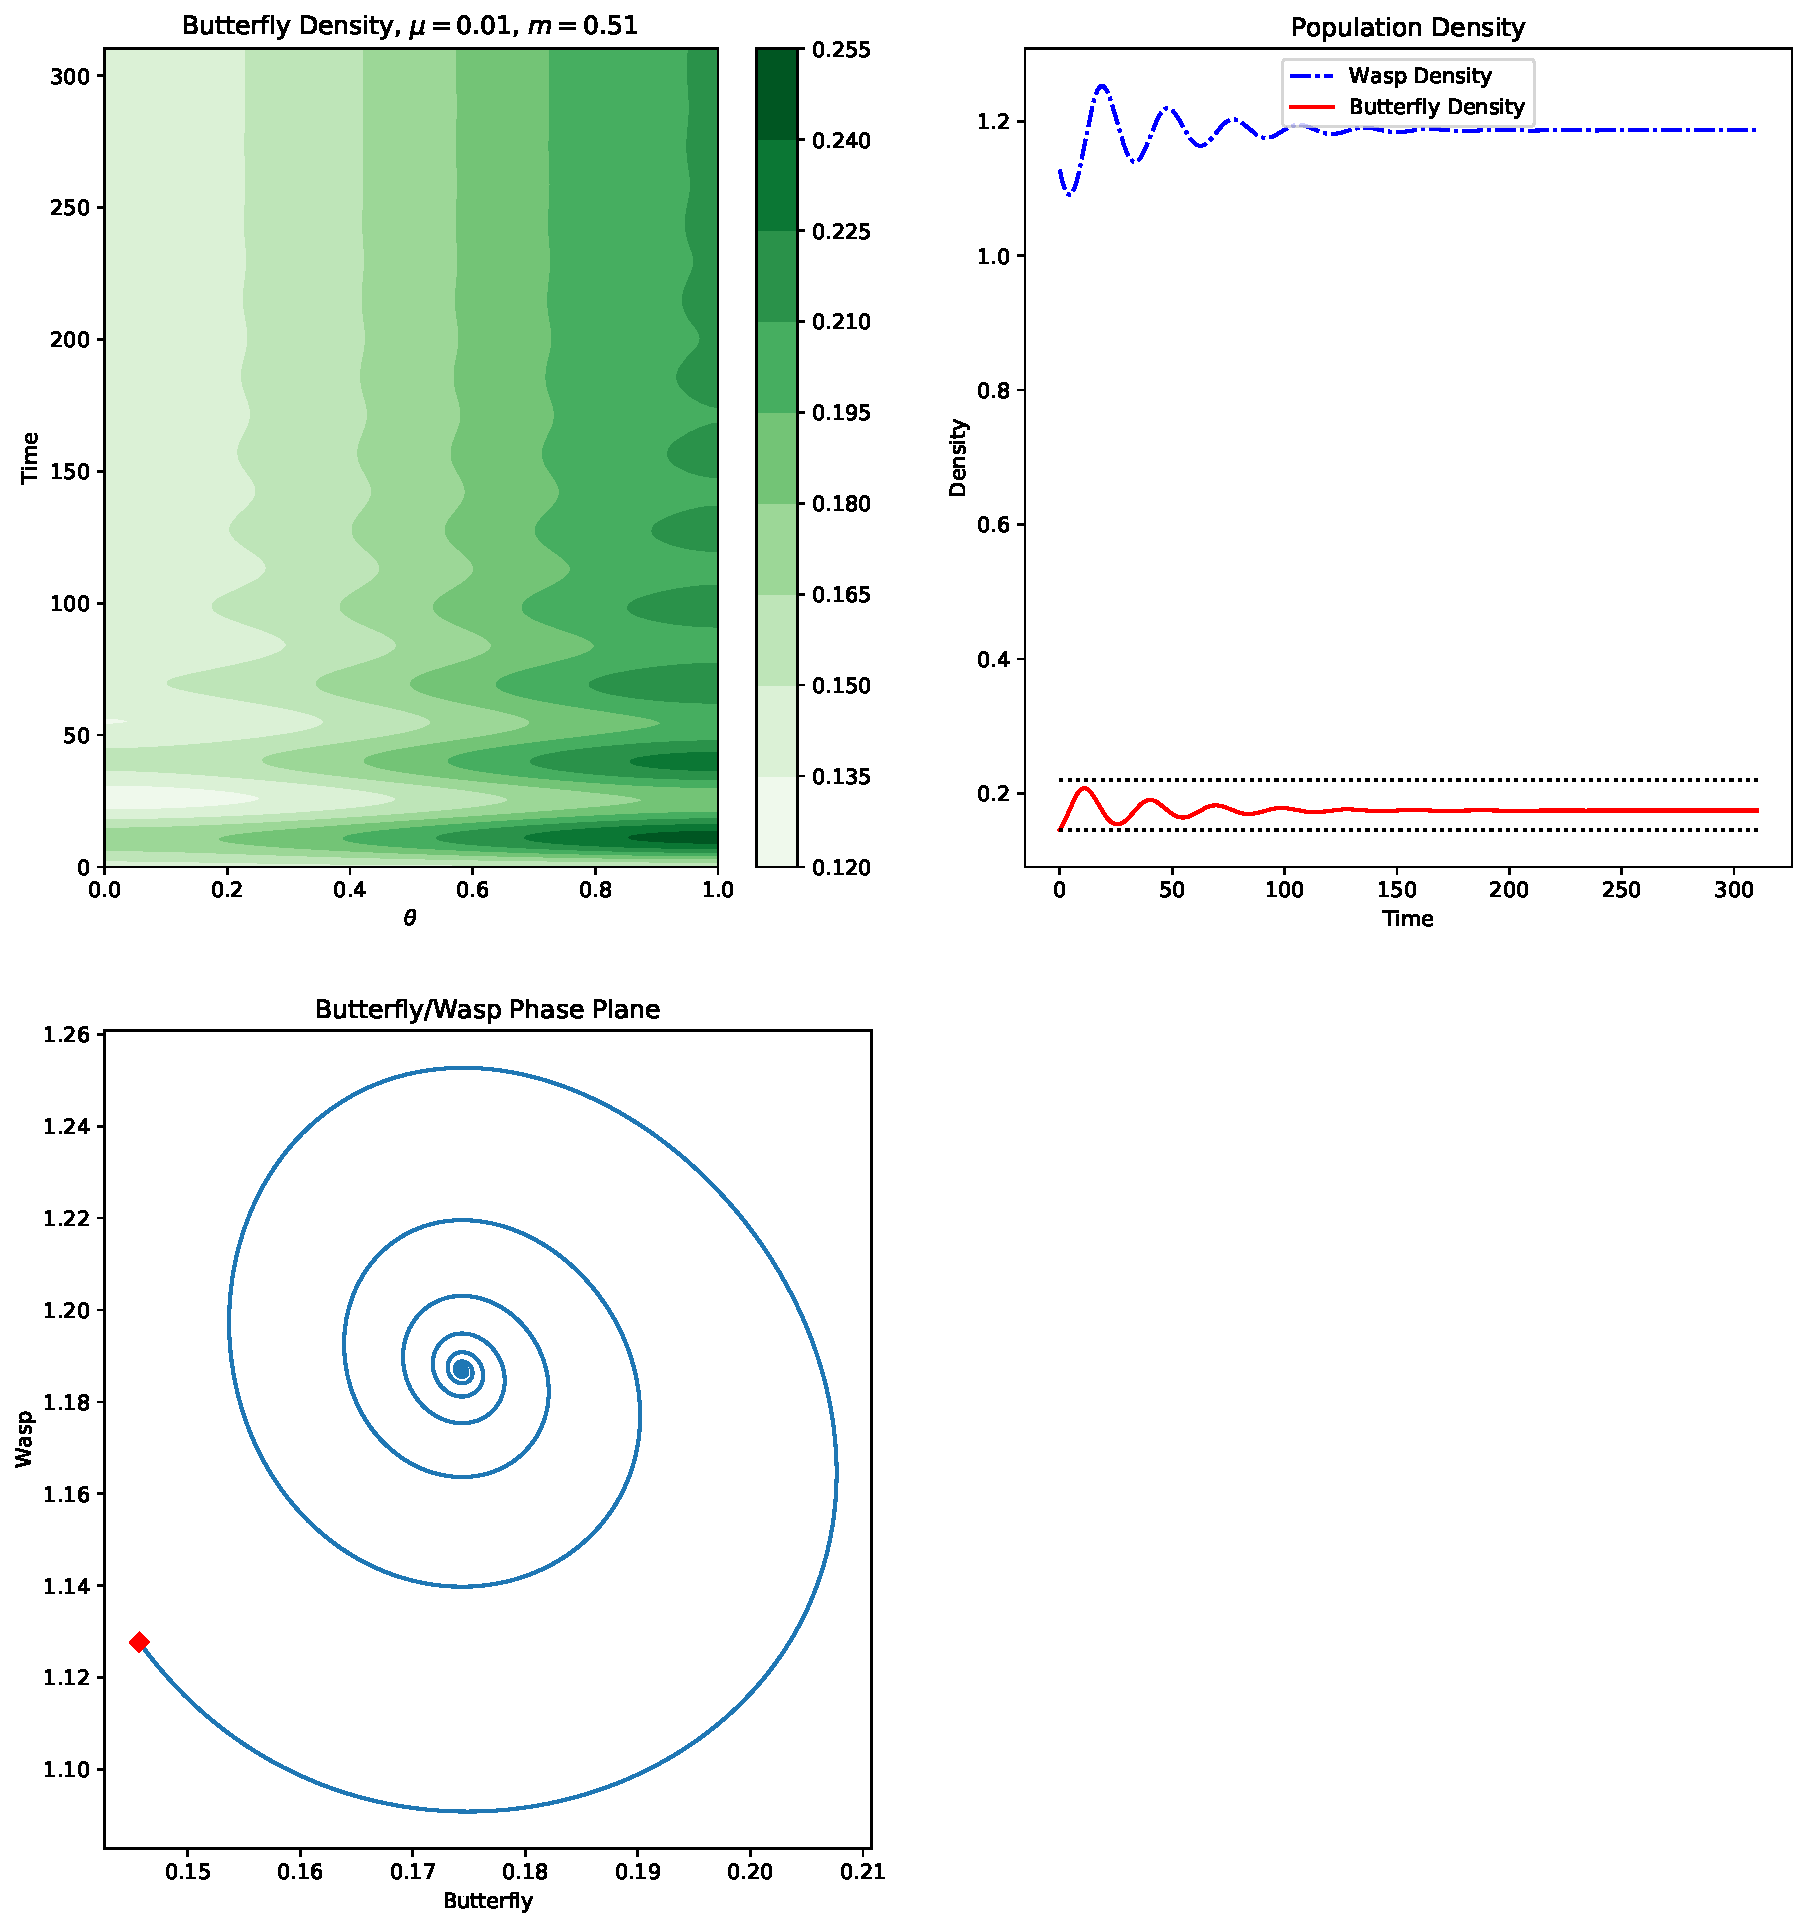
\includegraphics[width=12cm]{FIGURES/approximation-c-11-mu-01-m-51.pdf} \\
%   C & 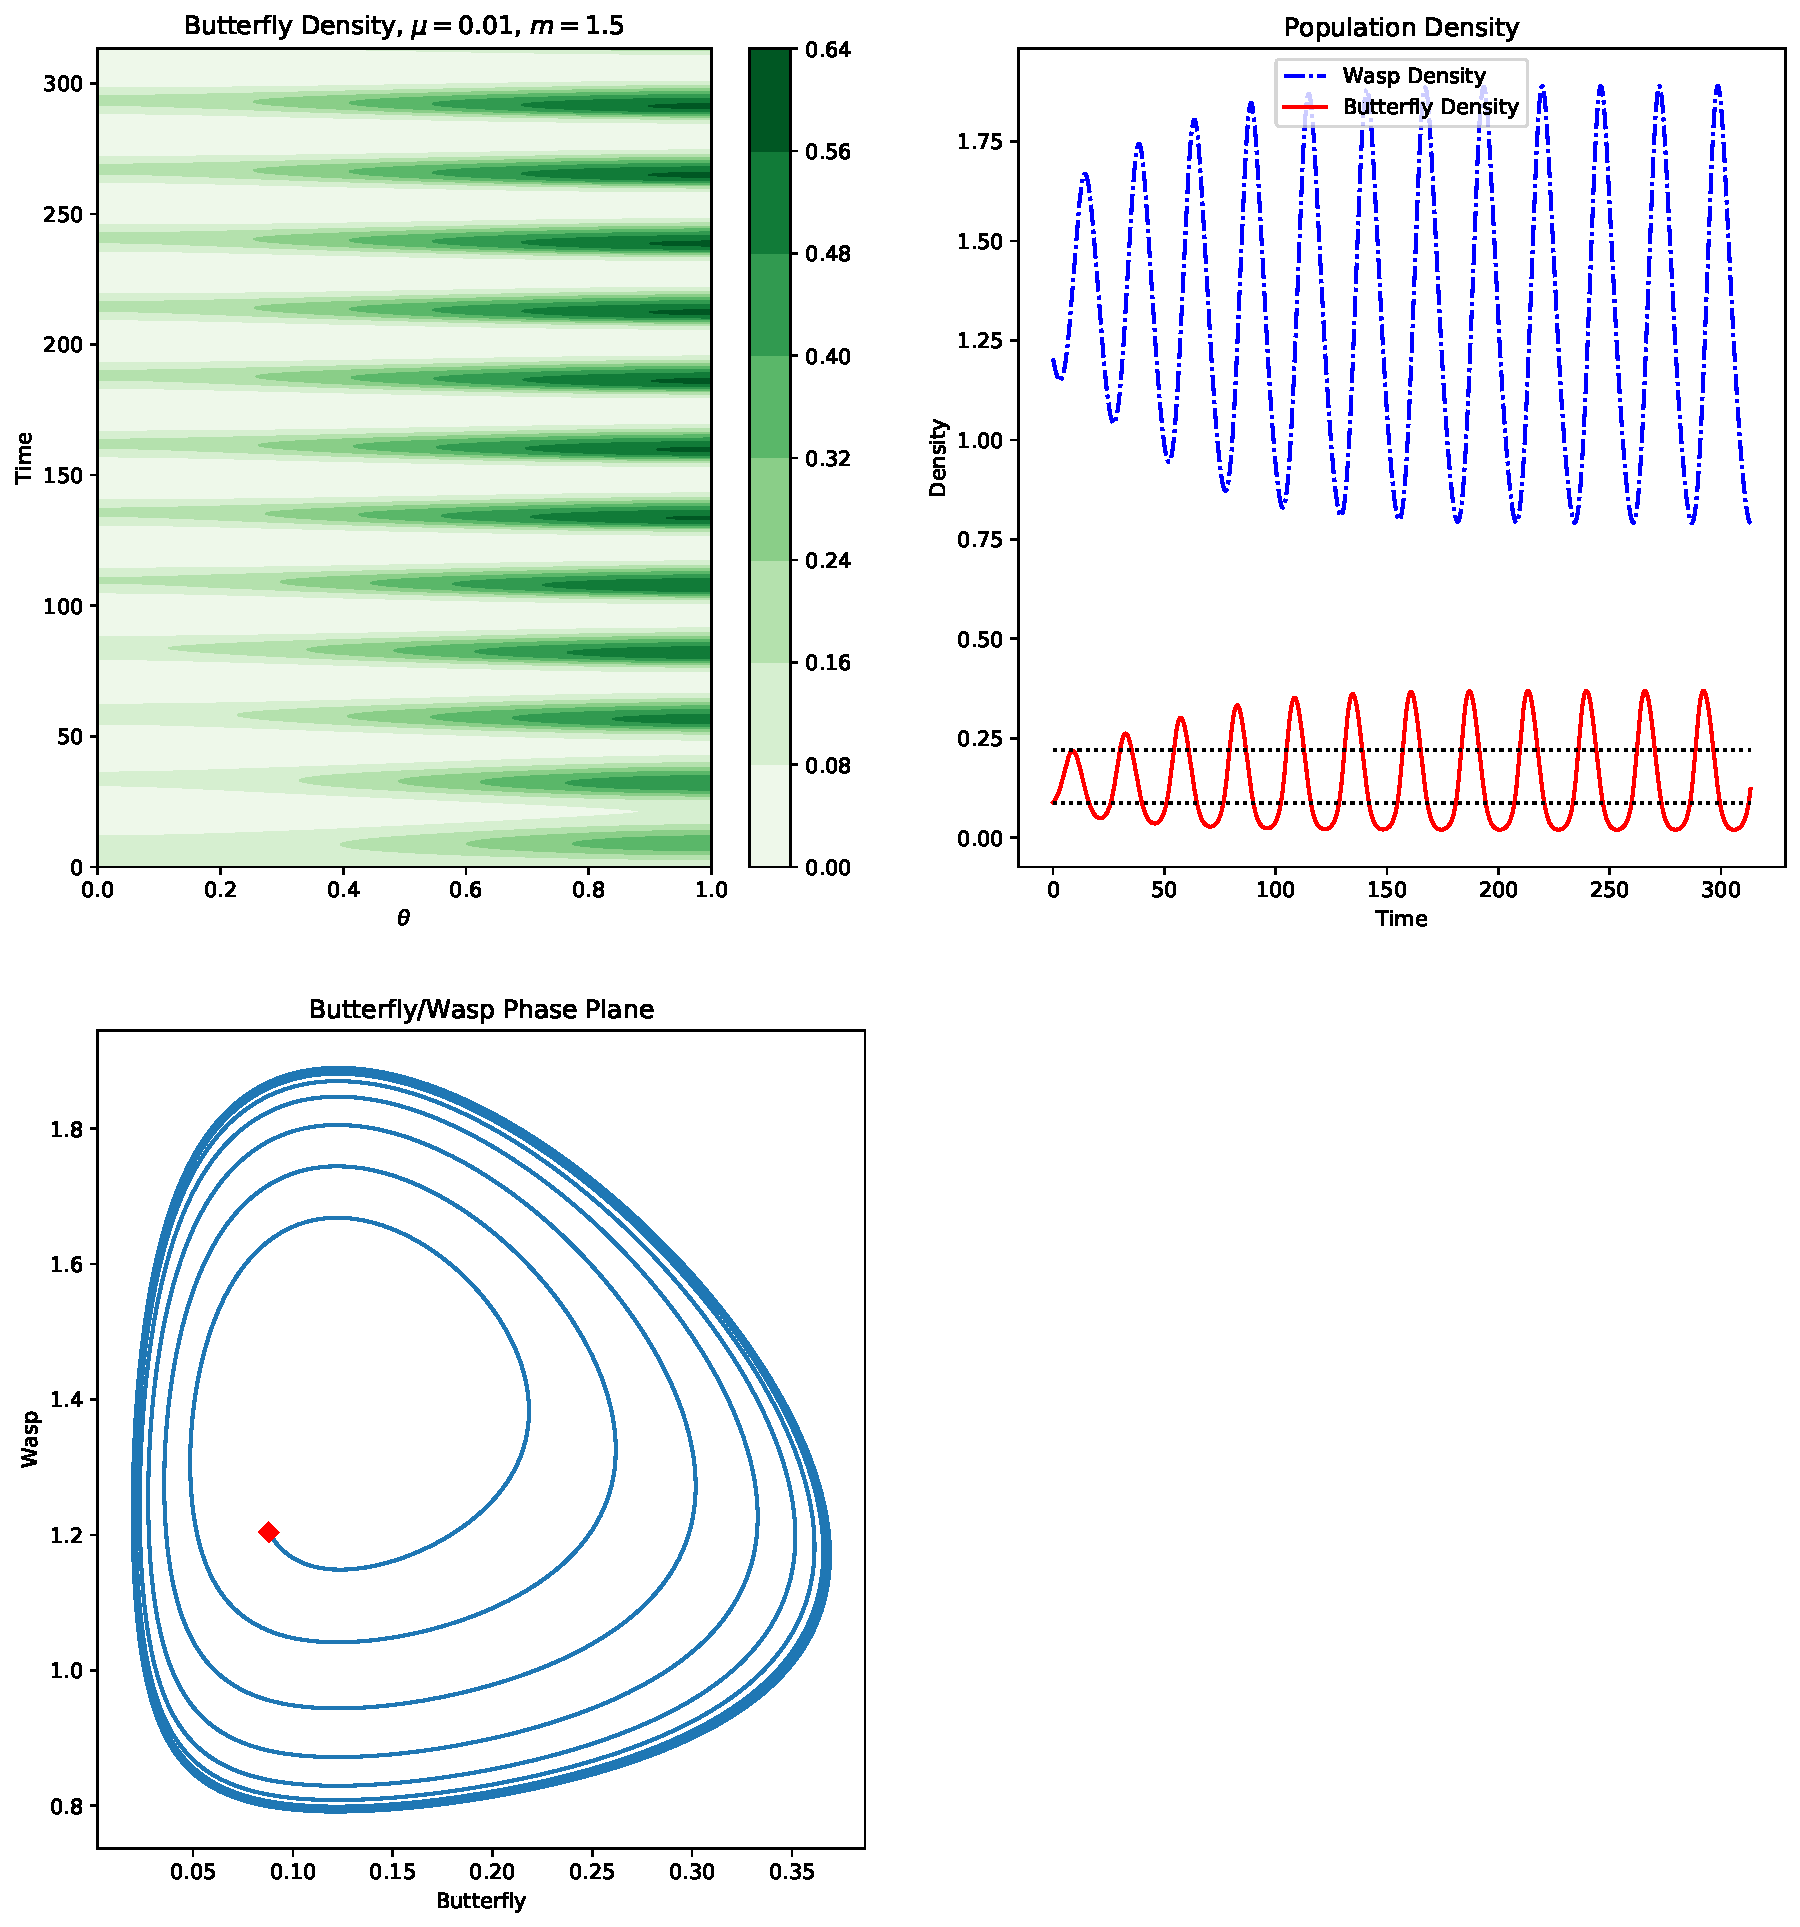
\includegraphics[width=12cm]{FIGURES/approximation-c-11-mu-01-m-150.pdf} \\
%   D & \includegraphics[width=12cm]{FIGURES/approximation-mu-01-m-12.pdf} \\
%   \end{tabular}
%\caption[Example of four approximations to the distributed system.]{Four %approximations to the distributed system are shown.}
%  \label{fig:distributedApproximations}
%\end{figure}


\begin{figure}[htb]
  \begin{tabular}{p{0.5\textwidth}p{0.5\textwidth}}
  \includegraphics[height=8cm]{FIGURES/maxMinByM-c-1.1-mu-01-04.pdf} 
  &
  \includegraphics[height=8cm]{FIGURES/maxMinByM-c-2.8-mu-01-04.pdf} \\
  \multicolumn{1}{c}{(A)} & 
  \multicolumn{1}{c}{(B)} \\
  \end{tabular}
  \caption[Upper and lower bounds of the butterfly density.]{The  upper
    % https://www.overleaf.com/project/5eb9da10e929ab0001816b1e
    and lower bounds of the long term density of the butterfly
    population. The dotted line shows the bounds for the ODE model, and the symbols are for the distributed model with different diffusion values. The population was approximated for different values
    of $\origM$. The approximation was stopped if it either became close to
    a steady state or a limit cycle.  The value of $g$ is 0.6, $d$ is 0.1. The value of $c$ for the graph on the left (A) is 1.1, and the value of $c$ for the graph on the right (B) is 2.8. The transition from stable to oscillatory solutions for the ODE occurs around $m\approx 0.5$ in graph (A) while in graph (B) it occurs near $m\approx 2.9$.   These transitions occur at higher values of $m$ for the distributed model.}
  \label{fig:odepdeButterflyMaxMin}
\end{figure}






\subsection{Numerical results for the system of ODEs}
\label{subsection:odeApproximation}

The long term stability of the system of ordinary differential equations given in 
equations (\ref{eq:scaledODE1}) and (\ref{eq:scaledODE2}) has been described in the previous subsection. In this subsection we explore the amplitude of oscillations where they occur. In particular, for some parameter values, the butterfly population density is close to zero over some time intervals, making extirpation likely. We also examine how the existence and amplitude of the oscillation depends on the parameters $\origM$ and $c$. The parameter $\origM$ governs the intensity of the impact of the use of the anti-aphrodisiac while $c$ governs the level of predatory pressure with an increase in $c$ resulting in a decrease in the predatory pressure of the wasps on the butterflies.



We begin with an exploration of how the butterfly population depends on $\origM$ while $\origC$ remains fixed by using the numerical solutions of the ODE model.
The dotted lines in graphs (A) and (B) in Figure \ref{fig:odepdeButterflyMaxMin} represent the maximum and minimum values of oscillatory solutions as $\origM$ varies  for $c=1.1$ and  $c=2.8$, respectively  (see  \ref{numericalApproximationODE} for details on the numerical solution). For small values of $\origM$ the system converges to a stable fixed point (single dotted line). As $\origM$
increases the solutions oscillate in a limit cycle. Further increasing $\origM$ results in a limit cycle in which the lower bound of the butterfly population gets close to zero creating a greater risk for population extirpation.


Comparing Figure \ref{fig:odepdeButterflyMaxMin}A and Figure \ref{fig:odepdeButterflyMaxMin}B, we see that the impact of increasing the value of $c$ is the shift to a larger value of $\origM$ where limit cycles first appear. In other words, lower predatory pressure decreases the tendency of the populations to oscillate.
This result is expected as we have previously shown in Section 4.1 that the bifurcation to oscillatory solutions appears at 
\begin{eqnarray}
\label{eqn:transitionLocation}
\origM^* & = & \left(\frac{g+d}{g-d}\right)c -1.
\end{eqnarray}
Therefore, as $c$ increases the transition  occurs at a larger value of $\origM$ and oscillatory solutions persist for all values of $\origM$ larger than $\origM^*$. In the next subsection we will compare this to the numerical results for the distributed model.


\subsection{Numerical Results for the distributed model}
\label{subsection:pdeApproximation}

In this subsection we provide a  numerical exploration of the distributed model, the coupled ODE and PDE system, equations (\ref{eq:scaledodePDE1}) and (\ref{eq:scaledodePDE2}). The details of the numerical solution method are
described in  \ref{numericalApproximation}.
To investigate the robustness of the results with
respect to initial conditions
 for the various trials, different initial conditions have been examined. 
We first conducted trials using initial conditions in which the majority of the population exhibits a higher propensity for using the pheromone.
Other choices included initial conditions based on a Gaussian function whose parameters minimized the residual from the steady state as well as initial conditions based on the steady state of a linearized distributed model. In all cases, the long term temporal behaviour was the same, and we did not observe any differences in the final outcomes.
 For the numerical results presented here, initial conditions in which the majority of the population exhibits a higher propensity for using the pheromone were used. 

We first focus on how the variance of animal behaviours, characterized by the change in the parameter $\origM$, impacts the long term behaviour of the system.
From our initial examination of the stability of the ODE system, as shown in Figure \ref{fig:distributedLineSegment}, the stability region depends on the parameter $\origC$, and we vary this parameter in the distributed system as well.
The parameter
range chosen for numerical investigations is consistent with that examined in subsection
\ref{subsection:odeApproximation}. 
We find that depending on the parameter regime, the system exhibits two types
of behaviour: a) both the butterfly and wasp populations reach a constant equilibrium or b) both populations
display periodic behaviour (see Figures \ref{fig:odepdeButterflyMaxMin} and \ref{fig:m-c-behaviours}). When comparing these results to the ODE model, it is important to note how the entire population of the butterflies impacts the dynamics, as the population's dynamics can vary in $\theta$. For example, the population of butterflies that highly utilize the anti-aphrodisiac may oscillate over time, and the ones that express the anti-aphrodisiac at a lower level may oscillate with a much lower amplitude. Conversely, the population of butterflies that  under-utilizes the anti-aphrodisiac may get close to zero while the parts that highly utilize the anti-aphrodisiac may reach a higher steady state population density. Some examples of these types of outcomes present in the distributed model are shown in Figure \ref{fig:m-c-behaviours} (Panels A-D).

\begin{figure}[!htp]
\begin{center}
\includegraphics[scale=.6]{FIGURES/Panel_figure.eps} 
\end{center}
\caption{In the top panel, we show the region of long-term oscillations for the butterfly density versus stable steady state in the $\origM$-$\origC$ plane. Each solid curve defines the boundary between oscillations and stable steady states in the distributed model for different $\mu$ values while the dashed line defines the same boundary for the ODE. Oscillations occur below the curves (smaller values of $c$) with respect to the distributed model while stable steady states occur above. The ODE model, on the other hand, exhibits oscillations to the right of the dashed line and stable steady states to the left.  The bottom panels A-D show the butterfly population distribution across $\theta$ in addition to the temporal dynamics of the total population of the PDE system for various values of $\origM$, and fixed value of $c=2$, $\mu=0.01$, $g=0.6$, and
$d=0.1$.}
\label{fig:m-c-behaviours}
\end{figure}

We first compare how the behaviours between the ODE and the distributed models vary with different values of the parameter $\origM$, which controls the slope of the impact function $p(\theta)$. In this way, a higher $\origM$ value corresponds to larger differences in the manifestation of the trait within a population, as well as a larger range of behaviour. In the ODE system, there is no dependence on $\theta$, therefore choosing a particular value of $\origM$ corresponds to keeping the propensity ($p=1+m$) for the use of anti-aphrodisiac fixed for the entire population. 


\begin{figure}[!htp]
\includegraphics[scale=0.4]{FIGURES/Total_change.jpg} 
\caption{The long term behaviour of the numerical solutions for the distributed system are examined.
The figures at the top (A and B), show the minimum long term butterfly densities at $\origTheta=0$ and $\origTheta=1$ for different values of the parameters $\origM$ and $\origC$. The figures on the bottom (C and D), show the maximum long term butterfly densities at $\origTheta=0$ and $\origTheta=1$ for different values of the parameters $\origM$ and $\origC$.   All runs use a value for the diffusion of $\mu=0.01$. Differences between the top and bottom figures indicate parameter ranges in which the solutions exhibit oscillatory behaviour. In both cases, $\origTheta=0$ and $\origTheta=1$, the only region in which oscillations occur in the long term behaviour is in the small ``hump'' that appears for smaller values of $\origC$ and $\origM$.}
\label{fig: 10percent_change}
\end{figure}

We find that for increasing values of $\origM$ the emergence of limit cycles is delayed or can be avoided altogether in the distributed model, as shown in Figures \ref{fig:odepdeButterflyMaxMin}, \ref{fig:m-c-behaviours} and \ref{fig: 10percent_change}. 
We note that the behaviour with respect to oscillations is less advantageous for the population as the population gets close to zero, therefore making extirpation more likely (see the minimum densities in Figure \ref{fig:odepdeButterflyMaxMin}, Figure \ref{fig:m-c-behaviours}C and Figure \ref{fig: 10percent_change}A and \ref{fig: 10percent_change}B) in the presence of fluctuations due to external influences. Increasing $\origM$ allows the system to escape oscillations altogether and revert back to a steady state, bounded away from zero for the individuals that utilize the anti-aphrodisiac the most (Figure \ref{fig: 10percent_change} B and D). We note that while the population is able to escape oscillations and stay bounded away from zero, it is only the butterflies with a higher propensity for expressing the trait that remain (see Figure \ref{fig: 10percent_change}). 

The ecological implication of this is that in the presence of variation, the range of the trait impact ($\origM$) plays
a role in the dynamics and helps the population remain at a constant equilibrium, bounded away from zero, and escape less advantageous oscillatory behaviour than it would otherwise exhibit in the absence of variation. However, this happens at the expense of the
sub-population of butterflies that does not display the trait as strongly.

\par Further, we also investigate how these results change as we vary the diffusion coefficient $\mu$ in the distributed model, which represents the rate at which the change in the group phenotype composition happens from generation to generation. 
We find that as $\mu$ increases, the oscillatory region increases and a larger value of $\origM$ is needed to bring the population back from an oscillatory state to a steady state (see the top most image in Figure \ref{fig:m-c-behaviours}).  
We also note that as $\mu$ increases, the results more closely resemble those of the ODE system. This is expected as faster changes in the group phenotype composition lead to a more well-mixed population. The population as a whole is relatively uniform with respect to $\theta$ and should more closely resemble the ODE system where there is no dependence on $\theta$. Higher diffusion results in more rapid mixing throughout the population allowing subsets of the population to be mixed more rapidly. If a rapid fluctuation begins in one part of the population, corresponding to a specific level of anti-aphrodisiac use, a greater diffusion will result in a quicker redistribution of the population with respect to  $\origTheta$. 
%In many cases, spatially explicit population models tend to be more stable, with less tendency for extirpation, compared to ODE models that exclude animal movement. Allowing individuals an opportunity to seek refuge is one reason enhancing stability \citep{levins1969some}. Similarly, implementing explicit variation for group phenotype composition appears to have an analogous effect on stability. 

We also find that the choice of the parameter $c$ plays a role in the dynamics. In the case of low predatory threat (higher values of $c$), group variation does not have as great
of an impact on population dynamics as the population is able to remain at a constant equilibrium, free of oscillations, regardless of the choice of $\origM$. We note that for smaller values of $c$, the dynamics of the distributed model more closely resemble those of the related ODE system, with the exception of the fact that in the distributed model, increasing the value of the parameter $\origM$ has the ability to cease oscillations and return the system to a stable steady state (see Figure \ref{fig:odepdeButterflyMaxMin}A).





%\begin{figure}[!htp]
%\begin{center}
%\includegraphics[scale=0.6]{FIGURES/m_vs_c_new.png} 
%\end{center}
%\caption{REMOVE**Selection of simulations in the $m-c$ parameter %space for various values of $\mu$. Latin Hypercube Sampling is used to %generate N=300 sets of samples from the $m-c$ parameter space. For each %pair of parameter values, the PDE was integrated using the explicit finite %difference method. For each pair, we classify the long-term behaviour as %either oscillatory (red) or constant steady state (blue), and whether the %butterfly density gets close to zero (circle) across all $\theta$s, stays away %from zero for across all $\theta$s (diamond) or stays away from zero for %only the upper range of $\theta$s (cross). 
%Further, considering only the second half of the time domain (to exclude %possible transient behaviour), the 80th percentile of theta values was used %to determine the maximum butterfly density ($B_{high\theta}$). For the %same time slice, the 20th percentile of theta values was used to determine %the maximum butterfly density ($B_{low\theta}$). For each pair of %parameter values, we calculate $\frac{B_{high\theta}}{B_{low\theta}}$ %and express this ratio on the log scale.  In this way, a negative value of the %log of the ratio is indicative of a population where most of it is %concentrated at the lower values of $\theta$. For values of exactly 0, the %population is evenly distributed with respect to $\theta$. Anything above %0 indicates that most of the population is concentrated at the high values %of $\theta$. We used the MATLAB function \textit{scatteredInterpolant} %to interpolate and plot the ratios as a heat map with lighter areas %corresponding to higher values of the ratio.}
%\label{fig:m_vs_c}
%\end{figure}






%\begin{figure}[!htp]
%\begin{center}
%\includegraphics[scale=0.6]{FIGURES/totalChange-tenP-mu-0.1} 
%\end{center}
%\caption{The temporal changes of the distribution of butterflies. Two points in the domain, $\theta$, were monitored during the approximation of the coupled system. One point was near $\theta=0.1$ (left side) and the other near $\theta=0.9$ (right side). Once the approximation settled into either a repeating solution or a steady state the maximum and the minimum of the butterfly population was recorded over a full cycle if the solution repeated, otherwise the value at the steady state was recorded. The dotted line represents the location of the transition between a stable solution and a limit cycle in the ODE system. }
%\label{fig:temporalChange_m_vs_c}
%\end{figure}

%\begin{figure}[!htp]
%\begin{center}
%\includegraphics[scale=0.6]{FIGURES/Simulations_mu_0.04.eps} 
%\includegraphics[scale=0.2]{FIGURES/Ratio_mu0.01.jpg}  
%\end{center}

%\caption{Figure A shows a selection of runs in the $m-c$ parameter space for $\mu=0.04$. Figure B shows the $m-c$ parameter space for $\mu=0.01$. Low values of c correspond to a high-predation scenario, where wasps receive the most benefit from butterfly consumption. The parameter $\origM$ corresponds to the variation of the trait manifestation within the butterfly population. Three important observations: 1) In the presence of higher variation of the trait in the butterfly population, the "strong" survive at the expense of the weak (the level of predation still plays a role here, too).
%2) The oscillations of the wasp population get close to zero in the low-c region. This may be due to the length of the cycle in the butterfly population (as compared to the scenario in the higher-c region). The wasps don't have enough time to recover from a rapid collapse of the butterfly population. 
%3) As $\mu$ decreases, the idea of how the butterflies that display the trait at a greater rate  (higher $\theta$)  surviving at the expense of those that are less likely to display the trait is more clearly observed. This should make sense as lower $\mu$ corresponds to less homogeneous populations, which remains so for longer (the trait distribution changes slowly from generation to generation) 
%4) May be worth exploring and framing in the context of "realistic" versus "ideal" region?
%}
%      \label{fig:mvsc}
%\end{figure}

\section{Conclusion}

%\begin{figure}[!htp]
%\begin{center}
%\includegraphics[scale=.4]{FIGURES/Bifurcation_2d.eps} 
%\end{center}
%\caption{Region of oscillations versus stable steady state in the $\origM$-$c$ plane. Oscillations occur below the curves (smaller values of $c$) while stable steady states occur above. The curves are given for different values of the diffusion coefficient, $\mu$. }
%\end{figure}



 A number of investigators have noted the impact of behavioral variation within a population on the dynamics of the population as a whole. As the number of possible expression levels associated with the trait grows,  the complexity associated with the analysis of the resulting model systems can grow prohibitively difficult. The framework proposed here provides a novel approach for modeling the behavioural variation in a population as a continuous distribution. We use a diffusion process to model the temporal dynamics of the distribution. The proposed modeling approach provides an alternative way to model the variation in animal behaviour using a time varying continuous distribution, which has not previously been done, to our knowledge. 
 
If variations in behaviour are represented as compartments in an ODE model, then a continuous distribution and a compartment-based approaches are consistent for a sufficiently large number of levels. For this model, that sufficient number was approximately 40, meaning that in terms of model size and complexity, accurate representation of behaviour requires about a 20-fold increase in the number of equations (see Figure \ref{fig:comparisonDistributedCompartments} and  \ref{appendix:compartmentModels} for further details.) Therefore, one advantage of our model and the use of a continuous representation of behaviour is the ability to refine the resolution and include a greater number of levels representing the different manifestations of an animal's behaviour. In addition,  it provides a context to make use of qualitative methods to analyze partial differential equations to examine stability, sensitivity, transport phenomena, and other spatio-temporal dynamics.
 

 
  In the work presented here we first compared the related ODE system (which excludes variation in the phenotype) and the distributed model. The ODE system is more mathematically tractable, and we used insight gathered from its analysis to inform our numerical investigations of the distributed model. The ODE model does not take into consideration the variation in the behaviour and does not give a full picture, highlighting the importance of including variation in the modeling process. One of the key results from the comparison of the two approaches is that the onset for the transition to a limit cycle is delayed, or can be avoided altogether, for certain values of key parameters. In particular, a sufficiently large value of the parameter $\origM$ (the range of the trait’s impact) in the distributed model can actually bring the population out of the oscillatory range and into an equilibrium state, bounded away from zero. This is not the case in the ODE model, which predicts solely oscillatory behaviour above a certain value of $\origM$. The ecological implication of this is that 1) group variation plays an important role in the dynamics of the system as reported in other studies \citep{doi:10.1111/j.1461-0248.2010.01536.x} and 2) given a large enough amount of variation within a group, the population can escape a less advantageous oscillatory state with critically low population numbers and continue its existence. However, this happens at the expense of the sub-population of butterflies that does not display the trait as strongly, as it is only those butterflies in our model that display the trait that survive.
  
  The trend in which the oscillations cease for increasing $\origM$ in the distributed system represents a departure from the predicted behaviour in the system of ODEs. In the system of ODEs the oscillations will occur for all values as $\origM$ increases. This result raises implications for other phenomena. For example, it has been noted that data collected from biological systems does not always confirm predictions of complex dynamics and requires careful analysis \citep{Skinner1994}.  
  %The resulting restriction in the range of parameters demonstrated here in which oscillations occur in the distributed system provide insights into additional possible reasons that chaos is difficult to detect from data obtained from observations of biological systems. 
 
The rate at which the the group phenotype diffuses throughout the population  from generation to generation (given by $\mu$), also has a significant impact on the results discussed above. As $\mu$ increases, the oscillatory region increases and a larger amount of variation within a group (larger values of $\origM$) is required to bring the population back from oscillatory state to a steady state.  Further, as $\mu$ increases, the results start to resemble those of the ODE system. This is expected as faster exchange within the group phenotype composition lead to a more well-mixed population and therefore should resemble the ODE system  in which variation is not accounted for. Allowing explicit variation for group phenotype appears to promote a system that tends to a stable steady state, similar to how spatially explicit population models which allow for animal movement tend to be more stable \citep{levins1969some}.

Finally, the trends in the previously mentioned dynamics were more pronounced in the case of high predatory threat (low values of $c$). In the case of low predatory threat, group variation does not have as great of an impact on population dynamics as the population is able to remain at a constant equilibrium.  This suggests that while a higher degree of group variation may benefit the overall population and help it avoid extirpation in the presence of severe predatory pressure, it has no clear advantage when the predatory pressure is low.

One limitation of our model is the lack of understanding the realistic ranges for the various parameters. We investigated an extensive parameter space and the behaviours that were possible within it. In the future, the model could be calibrated using parameters better informed by experimental data. Also, the wasps modeled in our paper predate several hosts, and incorporation of alternate butterfly hosts would provide an ecologically relevant extension to our model. The model presented here will also benefit from a further examination of a non-trivial, non-linear propensity function, $p(\origTheta)$. For example, the benefit associated with some behaviours may diminish as the strength of the trait increases. In addition, it would be beneficial to examine the use of different propensity functions associated with the different terms in the model.

 
As interest in behavioral differences within populations continues to grow, the approach presented here provides an alternative way to model the impact of behavioral variation on the dynamics of a population. The modeling approach presented here addresses an important question regarding the role of variation in how a trait is expressed throughout a population and builds on previous efforts investigating this phenomenon \citep{doi:10.1111/j.1461-0248.2010.01536.x,doi:10.1086/687235,mierzejewski_horn_luong_2019}. The use of a diffusion process to model the spread of a trait through a population provides a novel approach to modeling behavioral variation that has several advantages.

%\section{Acknowledgements}

\vfill

This research did not receive any specific grant from funding agencies in the public, commercial, or not-for-profit sectors.

\clearpage

\appendix

\section{Stability analysis of the ODE system}
\label{appendix:otherFixedPoints}

In subsection \ref{subsection:parameters}, we examined the stability of the
non-trivial fixed point in the positive quadrant for the ODE system given by equations (\ref{eq:scaledODE1}) and
(\ref{eq:scaledODE2}). In this appendix we provide a more complete stability analysis for all fixed points of this system.  In particular  two other
fixed points are determined and the linear
stability at these two fixed points is discussed.

The  system of equations given in by
(\ref{eq:scaledODE1}) and (\ref{eq:scaledODE2}) has at most one fixed point
with both $b>0$ and $w>0$.  As discussed in \ref{subsection:parameters}, $b^*= \frac{dc}{(g-d)p}$ and $w^* = (c+\frac{dc}{g-d})(1- \frac{dc}{(g-d)p}).$  There are two other fixed points on the boundary of the positive quadrant, at $(b,w)=(0,0), \,(0,1)$. 
  

The stability at these two fixed points can be examined by first
determining the Jacobian of the system,
\begin{eqnarray*}
  J & = & \left[
          \begin{array}{rr}
            J_{11} & J_{12} \\
            J_{21} & J_{22}
          \end{array}
          \right].
\end{eqnarray*}
The entries of the matrix are given by
\begin{eqnarray*}
  J_{11} & = & p(1-2b) -
               \frac{w  c   p}{\left( c + pb \right)^2}, \\
  J_{12} & = & -\frac{pb}{c+pb}, \\
  J_{21} & = & g \cdot\frac{wcp}{(c+pb)^2}, \\
  J_{22} & = & -d + g  \cdot \frac{pb}{c+pb}.
\end{eqnarray*}

For the fixed point at the origin, the Jacobian reduces to 
\begin{eqnarray*}
  J~\bigg|_{(0,0)} & = & \left[
          \begin{array}{rr}
            p & 0 \\
            0 & -d
          \end{array}
          \right].
\end{eqnarray*}
Since it is assumed that both $p$ and $d$ are non-negative, this fixed point  is unstable  (saddle point).



At the fixed point $b=1$, $w=0$, the Jacobian is given by 
\begin{eqnarray*}
  J~\bigg|_{(1,0)} & = & \left[
          \begin{array}{cc}
            -p & -\frac{p}{c+p} \\
            0 & -d+\frac{gp}{c+p}
          \end{array}
          \right].
\end{eqnarray*}

This fixed point is unstable as long as $\left( \frac{g-d}{d}\right)p >c$.  This condition is equivalent to $w^*>0$.  (If on the other hand, $\left( \frac{g-d}{d}\right)p <c$, then the equilibrium $(b^*,w^*)$ moves into the fourth quadrant ($w^*<0$) and the equilibrium $(1,0)$ is a stable fixed-point.)


\noindent
\textbf{Limit Cycles}

In \ref{subsection:parameters} we showed that there is an equilibrium solution $(b^*,w^*)$ in the positive quadrant for the ODE system under the conditions:  1.)  $g-d>0$, and 2.) $c<\left( \frac{g-d}{d}\right)p$.   Here, the values of  $p$ are constrained by $1<p<1+m$.   We also showed in that section that this 
equilibrium is stable if and only if $\left( \frac{g-d}{g+d}\right)p < c.$   In this appendix, we prove the existence of a limit cycle when this latter inequality fails, i.e. the equilibrium becomes unstable.

We begin by remarking that the positive quadrant of the $(b,w)$-plane is invariant under the flow of the ODE system.

\begin{lemma}


All solutions of equations (\ref{eq:scaledODE1}) and
  (\ref{eq:scaledODE2}) with initial values
  $b\left( 0\right) > 0 ,w\left( 0\right) >0$ remain in the positive quadrant, $\mathbb R_+^2$, for all time.
\end{lemma}

\begin{proof}
  This follows by noticing that the non-negative axes, $\{(b,0):\  b \ge 0\}$ and $\{(0,w):\  w\ge 0\}$ are invariant under the flow, that is, if a solution starts in this set then it remains in this set. Then, by uniqueness, we conclude that no flow line can pass from the positive quadrant through these axes.
\end{proof}

We next show that all solutions in the positive quadrant are bounded for all positive time.  

\begin{lemma}
There exists $R_{0}>0$  such that for all $R\geq R_{0}$, the right
triangle, 
$$T_{R}=\left\{ \left(b,w\right) \in \mathbb R^{2}:\  b\ge 0, w\ge 0, \ {\rm and}\  b+\frac{1}{g}w\le R\right\}, $$  
is positively invariant.
\end{lemma}

\begin{proof}
  We first note that if for some $t_0$, $b(t_0)< 1,$ then $b(t) < 1$ for all $t>t_0$.  This follows from the fact that equation (\ref{eq:scaledODE1}) shows that 
  $$\frac{d}{dt}b(t) < 0,\  \  {\rm when}\ \ b(t)\ge 1.$$
  
  Now, since we have already discussed that solutions in the positive quadrant cannot cross the axes, it is only left to show that we can choose $R_0$ large enough so that if $R>R_0$, we have
  $$\frac{d}{dt}\left(b(t)+\frac{1}{g}w(t)\right) <0,\  {\rm when}\  b(t)+\frac{1}{g}w(t) =R.$$
  
  But from equations (\ref{eq:scaledODE1}) and (\ref{eq:scaledODE2}), we have
  $$\frac{d}{dt}\left(b(t)+\frac{1}{g}w(t)\right)  = p b(t)\left( 1-b(t)\right) -\frac{d}{g}
w\left( t\right) . $$

If $b(t) \ge 1$, the right hand side is negative.  On the other hand, if $b(t) < 1$, we use $\frac{d}{g}w(t) = d(R-b(t))$ to get
$$\frac{d}{dt}(b(t)+\frac{1}{g}w(t)) =p b(t)\left(
1-b(t)\right) -d\left( R-b(t)\right),$$
which is negative if $R>R_0= \frac{p}{d} +1.$
\end{proof}



\begin{theorem}
  If $0 < c < \left( \frac{g-d}{g+d}\right)p$, then there exists at least one  limit cycle solution to equations (\ref{eq:scaledODE1}) and (\ref{eq:scaledODE2}) in the positive quadrant.
\end{theorem}
\begin{proof}
This is a direct consequence of the Poincair\'{e}--Bendixson theorem \citep{nonlinearChaos}, used with the previous lemma.
\end{proof}
Summarizing these results, we have the following theorem. 

\begin{theorem}
  The system of ordinary differential equations given by equations (\ref{eq:scaledODE1}) and (\ref{eq:scaledODE2}) (with $g\ne d)$ has fixed points in the $(b,w)$-plane at the points $(0,0), (1,0),$ and $(b^*,w^*)$, where $b^*=\frac{cd}{p(g-d)}$ and
$w^*=\left(\frac{cd}{g-d}+c\right)\left(1-\frac{cd}{p(g-d)}\right)$. 
 The  fixed point $(b^*,w^*)$ lies in the positive quadrant if $g-d>0$ and $c<\left( \frac{g-d}{d}\right)p$.  Considering $c$ as a bifurcation parameter, the system undergoes a Hopf bifurcation at $c^* = \left( \frac{g-d}{g+d}\right)p$.  
That is, the fixed point $(b^*,w^*)$ is asymptotically stable when $c>\left( \frac{g-d}{g+d}\right)p$ and is unstable if $c<\left( \frac{g-d}{g+d}\right)p,$ and, since all positive solutions to the system are bounded,  there is   a  limit cycle in the positive quadrant when the fixed point is unstable.
Finally, the fixed point $(0,0)$ is always an unstable saddle point, and the fixed point $(1,0)$ is unstable when $c<\left( \frac{g-d}{d}\right)p$, otherwise it is stable.
\end{theorem}

%\section{Stability of the %Equilibria}
\label{appendix:stability}




\section{Relationship Between Compartment Models and The Distributed Model}
\label{appendix:compartmentModels}

One common method to derive a mathematical model of a system that exhibits behavioural variation is through the use of a compartment model.  
The basic idea is that the variation is represented using a discrete set of possible levels in which a particular behaviour can be exhibited.
Each level is then treated as one compartment in a system of ordinary differential equations. 
For example, each compartment associated with a subset of the butterfly population is governed by an ordinary differential equation similar to the one given in Equation (\ref{eq:initialSystem1}). 
The population of wasps is governed by an equation based on the sum of butterflies across all of the compartments, and it is similar to the one given in Equation (\ref{eq:initialSystem2}). The primary difference is the addition of terms to model the exchange between compartments.

The resulting equations take a basic form given by 
\begin{eqnarray}
  \label{eq:compartmentSystem1}
  \frac{d}{d\origT} \origB_i(\origT) & = & \origAlpha p(\theta_i) \cdot \origB_i(\origT) (\origK - \origB_i(\origT))
  - \origGamma \cdot \origW(\origT) \frac{p(\theta_i)\origB_i(\origT)}{\origC+p(\theta_i)\origB_i(\origT)} 
  + \mathrm{(Exchange~Between~Compartments)} \\ [20pt]
  \label{eq:compartmentSystem2}
  \frac{d}{d\origT} \origW(\origT) & = & -\origD \cdot \origW(\origT) + \origG \cdot \origW(\origT)
  \sum^N_{i=1} \frac{p(\theta_i)\origB_i(\origT)}{\origC+p(\theta_i)\origB_i(\origT)},
\end{eqnarray}
where $i=1,\ldots,N$ assuming there are $N$ compartments. $\origB_i$ is the butterfly density associated with compartment $i$ and $\theta_i$ is the value of the independent variable $\theta$ within compartment $i$. 

Our primary interest is to explore the system as the number possible levels associated with the behaviour grows larger. 
To do so, we assume that the range of $\theta$ is fixed and examine the trend for the system as the number of compartments increases.
We also assume that the exchange between compartments $b_i$ only occurs between nearest neighbors. 

Moreover, the rate of change depends on the difference between population densities of adjacent compartments. 
The motivation for this assumption is that if the population densities of two adjacent compartments is the same, then the exchange between compartments will sum to zero. The greater the difference in population densities, the greater the pressure for exchange between adjacent compartments to equalize the difference. For a compartment, $i$, whose associated value of $\theta_i$ is within the interior of the domain of $\theta$, $[\theta_{min},\theta_{max}]$, the rate of flow from compartment $i+1$ to  compartment $i$ is
\begin{eqnarray}
  \mu_N ( \origB_{i+1}-\origB_{i} ),
\end{eqnarray}
where $\mu_N$ is a constant of proportionality for a system with $N$ compartments. Similarly, the rate of flow moving from compartment $i$ to compartment $i-1$ is
\begin{eqnarray}
  \mu_N ( \origB_{i}-\origB_{i-i} ).
\end{eqnarray}
The total rate of flow into compartment $i$ is the difference between the two quantities,
\begin{eqnarray}
  \mu_N ( \origB_{i+1}-2\origB_i+\origB_{i-i} ).
\end{eqnarray}


The resulting model that arises from these assumptions is 
\begin{eqnarray}
  \label{eq:difference1}
  \frac{d}{d\origT} \origB_i(\origT) & = & \origAlpha p(\theta_i) \cdot \origB_i(\origT) (\origK - \origB_i(\origT))
  - \origGamma \cdot \origW(\origT) \frac{p(\theta_i)\origB_i(\origT)}{\origC+p(\theta_i)\origB_i(\origT)} 
  + \mu_N \left( \origB_{i+1}-2\origB_i + \origB_{i-1} \right) \\ [20pt]
  \label{eq:difference2}
  \frac{d}{d\origT} \origW(\origT) & = & -\origD \cdot \origW(\origT) + \origG \cdot \origW(\origT)
  \sum^N_{i=1} \frac{p(\theta_i)\origB_i(\origT)}{\origC+p(\theta_i)\origB_i(\origT)}.
\end{eqnarray}
Focusing on Equation (\ref{eq:difference1}), assuming a uniform distribution of the values of $\theta_i$, we get $\triangle\theta=\frac{\theta_{max}-\theta_{min}}{N}$. Equation (\ref{eq:difference1}) can be expressed as
\begin{eqnarray}
  \frac{d}{d\origT} \origB_i(\origT) & = & \origAlpha p(\theta_i) \cdot \origB_i(\origT) (\origK - \origB_i(\origT))
  - \origGamma \cdot \origW(\origT) \frac{p(\theta_i)\origB_i(\origT)}{\origC+p(\theta_i)\origB_i(\origT)} 
  + \mu_N \frac{(\theta_{max}-\theta_{min})^2}{N^2} \frac{ \origB_{i+1}-2\origB_i + \origB_{i-1}}{\triangle\theta^2}.
\end{eqnarray}
The difference quotient in the final term is a second order approximation of the second partial derivative of $\origB(\theta,t)$ with respect to $\theta$,
\begin{eqnarray}
  \frac{d}{d\origT} \origB_i(\origT) & = & \origAlpha p(\theta_i) \cdot \origB_i(\origT) (\origK - \origB_i(\origT))
  - \origGamma \cdot \origW(\origT) \frac{p(\theta_i)\origB_i(\origT)}{\origC+p(\theta_i)\origB_i(\origT)} 
  + \mu_N \frac{(\theta_{max} - \theta_{min})^2}{N^2} \left( \frac{\partial^2}{\partial\theta^2} b \bigg|_{\theta=\theta_i} + O(\triangle\theta^2)\right).
\end{eqnarray}
In order for the rate of exchange to remain bounded as $N$ changes, the term $\mu_N \frac{(\theta_{max}-\theta_{min})^2}{N^2}$ must be $O(1)$, in other words, $\mu_N$ should scale as $N^2$. This condition is necessary for the rate of diffusion between compartments to not grow arbitrarily as different number of compartments are used to represent the same behavioural variation.
As $N$ grows large Equation (\ref{eq:difference1}) will approach the PDE found within the distributed model in Equation (\ref{eq:initialSystem1}) as demonstrated in Figure \ref{fig:comparisonDistributedCompartments}. The potential interdependence between the rate of change between compartments and the number of compartments indicates that a numerical exploration of the dependence on the number of compartments within the system should be carried out with great care.



\begin{figure}[!htp]
\begin{center}
\includegraphics[scale=.55]{FIGURES/comparison_pde_compartments.eps} 
\end{center}
\caption{This figures demonstrates the lack of agreement between the ODE model and the distributed PDE model when the number of compartments is small. As the number of compartments representing the variation in behaviour increases, the solution of the distributed PDE model is qualitatively the same as that of the ODE model. The following parameters were used: $m=16, c=2, d=0.1, g=0.6$ and $\mu=0.01$. }
\label{fig:comparisonDistributedCompartments}
\end{figure}
\section{Numerical Approximations}
\label{numericalApproximationODE}
\subsection{Numerical Solutions of the ODE system}
The system of ODEs given in
equations (\ref{eq:scaledODE1}) and (\ref{eq:scaledODE2}) was
solved using the Runga-Kutta Fehlberg method with a minimum step
size of $10^{-5}$. 
The initial values of the butterflies and wasps
were taken to be 95\% of the values for the non-trivial steady state. The
solution was run until the state was not changing or
a limit cycle was reached. In particular, if both population densities did not
change more than $10^{-7}$ from a previous high or low value for over
2000 time steps, the solution was considered to have reached steady state. For the
limit cycle, if the minimum and maximum for both population densities were within
$10^{-7}$ of each other for two full cycles, then the solution was considered to have converged to a limit
cycle.

A sequence of approximations was used to create the diagrams in Figure \ref{fig:odepdeButterflyMaxMin}, and they were made in succession by changing the value of $\origM$. The first approximation was constructed for the lowest value of $\origM$, and when the approximation was finished the value of $\origM$ was incremented. The initial condition for the next trial was the final state of the previous approximation. To investigate the possibility of hysteresis, the process was verified by also starting with the largest value of $\origM$, and the value of $\origM$ was decremented between approximations.    The results were nearly
identical, and no hysteresis was detected.

\subsection{Numerical Approximations of the distributed model}
\label{numericalApproximation}

This section focuses on the numerical solution of the distributed model in equations (\ref{eq:scaledodePDE1}) and
(\ref{eq:scaledodePDE2}). For the full system, we make use of a
Legendre pseudo-spectral collocation
method \citep{spectralMethodsFluids,hesthaven_gottlieb_gottlieb_2007,gottlieb1977numerical}. First,
the butterfly density is discretized in $\theta$ as
\begin{eqnarray}
  \label{eqn:spatialDiscretization}
  b_N(t,\theta) & = & \sum^N_{i=0} \hat{b}_i(t) \phi_i(\theta),
\end{eqnarray}
where $\phi_i(\theta)$ is the Lagrange interpolant on the
$i$\textsuperscript{th} abscissa of the Legendre-Gauss-Lobatto
quadrature \citep{hesthaven_gottlieb_gottlieb_2007}.

The abscissa of the Legendre-Gauss-Lobatto quadrature are the zeroes
of the function
\begin{eqnarray}
  \psi(\theta) & = & \left(1-\theta^2\right) L_{N}'(\theta),
\end{eqnarray}
where $L_N(\theta)$ is the $n$\textsuperscript{th} Legendre
polynomial \citep{davis2007methods}.  The weights, $w_n$, associated
with the quadrature are identical to those described by
\citet{davis2007methods} as well as \citet{gaussQuadratureRules}. In our examples the quadrature is
approximated using the methods described by \citet{gaussQuadratureRules}.  Given $\psi(\theta)$, the Lagrange
interpolants can be calculated as
\begin{eqnarray}
  \phi_i(\theta) & = & \frac{\psi(\theta)}{\psi'(\theta)(\theta-\theta_i)}.
\end{eqnarray}
The function $\psi(\theta)$ coincides with the Legendre differential
equation, and the relationship can be simplified as
\begin{eqnarray}
  \psi'(\theta) & = & -N(N+1)L_N(\theta).
\end{eqnarray}

The discretization of equations (\ref{eq:scaledodePDE1}) and
(\ref{eq:scaledodePDE2}) is constructed by substituting the definition
of $b_N$ from equation (\ref{eqn:spatialDiscretization}). A Galerkin
approximation is constructed, and one minor complication is that the
Lagrange interpolants are polynomials of degree $N$, and the
Gauss-Lobatto quadrature is exact for polynomials up to degree
$N$. The integral is approximated using the Gauss-Lobatto quadrature,
and the resulting sum results in an equivalent norm compared to the
Gauss quadrature which is exact for polynomials up to degree
$N$ \citep{SobolevCanutoQuarteroni}.

The resulting variational form for Neumann boundary conditions using a
Galerkin approximation and a discrete inner product for equation
(\ref{eq:scaledodePDE1}) is
\begin{eqnarray}
  \sum_{j=0}^N \sum_{i=0}^N  \hat{b}_i'(t) \phi_i(\theta_j) \phi_k(\theta_j) w_j
  & = &
  \sum_{j=0}^N \sum_{i=0}^N p(\theta_j)  \hat{b}_i(t) (1 - \hat{b}_i(t) ) \phi_i(\theta_j) \phi_k(\theta_j) w_j \\
  & &  -  \sum_{j=0}^N w(t) \frac{p(\theta_j) \sum_{i=0}^N \hat{b}_i(t) \phi_i(\theta_j) }{c+p(\theta_j) \sum_{i=0}^N \hat{b}_i(t) \phi_i(\theta_j)} \phi_k(\theta_j) w_j \nonumber \\ 
  & & - \sum_{j=0}^N \mu  \sum_{i=0}^N \hat{b}_i(t) \phi_i'(\theta_j) \phi_k'(\theta_j)  w_j, \nonumber
\end{eqnarray}
for all integer values of $k$ from $0$ to $N$ inclusive.  The basis
functions are the Lagrange interpolants on the abscissa, and the
equations can be reduced to
\begin{eqnarray}
  \hat{b}_k'(t) 
  & = &
        p(\theta_j) \hat{b}_k(t) (1 - \hat{b}_k(t) )
        -  w(t) \frac{p(\theta_k) \hat{b}_k(t)) }{c+p(\theta_k)  \hat{b}_k(t) }  
   - \frac{\mu}{w_k} \sum_{i=0}^N \hat{b}_i(t) \left( \sum_{j=0}^N  \phi_i'(\theta_j) \phi_k'(\theta_j)  w_j \right).
\end{eqnarray}
The corresponding discretization of the equation for the wasps can be simplified because the moth population is defined on the Gauss-Labotto points, and the integral can be approximated as described above. A similar approach has been described by \cite{doi:10.1002/mma.1318}.

Combined with equation (\ref{eq:scaledodePDE2}) the approximation
consists of a system of $N+2$ ordinary differential equations. The
integral in equation (\ref{eq:scaledodePDE2}) is approximated using
the Legendre-Gauss-Lobatto quadrature. The temporal discretization of
the resulting system is constructed using a second order, implicit
multi-step scheme. The scheme is implemented as a fully implicit
second order Adams-Moulton scheme \citep{ascher2011first}. At each time
step the resulting non-linear system is approximated using Newton's
method.



\clearpage
%\bibliographystyle{siam}
\bibliographystyle{elsarticle-harv}
\bibliography{animalBehaviour}



\end{document}

https://www.overleaf.com/project/5eb9da10e929ab0001816b1e